% ============================================================
% MAIN FILE — CMB Compatibility
% Target: JCAP
% ============================================================
\documentclass[a4paper,11pt]{article}
\usepackage{jcappub}

% --- Additional packages not provided by jcappub ---
\usepackage[utf8]{inputenc}
\usepackage[T1]{fontenc}
\usepackage{amsfonts}
\usepackage{booktabs}
\usepackage{array}
\usepackage[section]{placeins}
\usepackage{float}

\graphicspath{{figures/}}

% ============================================================

% --- Title ---
\title{CCR-Motivated Infrared Cutoff and CMB Power Spectrum Suppression}

% --- Authors and affiliations ---
\author[a]{N.~Chronis}
\author[b]{N.~Sifakis}

\affiliation[a]{Department of Computer Science \& Engineering,
  University of Crete, 70013 Heraklion, Greece}
\affiliation[b]{Department of Production Engineering and Management,
  Technical University of Crete, 73100 Chania, Greece}

\emailAdd{csd5174@csd.uoc.gr}

% --- Abstract ---
\abstract{We test the Conditional Cosmological Recurrence (CCR) framework against
Planck 2018 CMB data by identifying an infrared cutoff $k_c$ in the
primordial power spectrum from the finite Hilbert-space dimension $D$ of
the de~Sitter causal patch during inflation. The cutoff is not a free
parameter: it is a deterministic function of $D$ alone, fixed by the
Gibbons--Hawking entropy bound and standard thermal-history inputs. For
$\ln D \sim 10^{14}$, the predicted scale
$k_c \sim 10^{-4}\;\mathrm{Mpc}^{-1}$ falls in the window responsible
for the observed low-$\ell$ CMB power deficit. We implement the
CCR-modified spectrum in the CAMB Boltzmann code and constrain the model
parameters $\log_{10}(\ln D)$ and shape parameter $\alpha$ using Markov
Chain Monte Carlo sampling with Planck 2018 TT+TE+EE likelihoods. The data do not 
exclude the CCR framework but do not prefer it over $\Lambda$CDM: the Savage--Dickey Bayes
factor satisfies $|\ln B_{01}| < 1$, the BIC penalises the two extra parameters ($\Delta\mathrm{BIC} = +13$), 
and the posterior on $\ln D$ is approximately uniform over the prior range.
This null result is itself informative: it establishes that a $3\sigma$
detection requires $\ln D \lesssim 10^{13}$ (equivalently
$k_c \gtrsim 7 \times 10^{-4}\;\mathrm{Mpc}^{-1}$), a threshold
accessible to the combination of LiteBIRD polarisation and Planck
temperature data. The CCR framework simultaneously predicts the
tensor-to-scalar ratio $r = 16/(A_s \ln D)$, providing a two-observable
consistency test with future B-mode experiments.}

% --- Keywords ---
\keywords{CMB power spectrum; primordial power spectrum; inflation; infrared cutoff;
large-scale anomalies; Bayesian inference; holographic entropy}

% ============================================================
\begin{document}
\maketitle

% ============================================================
\section{Introduction}
\label{sec:intro}

% --- The low-ℓ anomaly ---
The angular power spectrum $C_\ell$ of the cosmic microwave background (CMB)
provides one of the most precise tests of the standard $\Lambda$CDM cosmological
model. At multipoles $\ell \gtrsim 30$, the agreement between the Planck 2018
observations~\cite{Planck:2018params} and the six-parameter $\Lambda$CDM
prediction is remarkable. At large angular scales ($\ell \lesssim 30$), however,
the observed power falls systematically below the theoretical expectation---a
deficit that has persisted across COBE, WMAP, and Planck data releases and is
robust across independent component-separation methods. The reconstructed
primordial power spectrum shows a $\sim 2\sigma$ suppression at
$k \lesssim 10^{-3}\,\mathrm{Mpc}^{-1}$~\cite{Planck:2018inflation}, and the
phenomenological infrared cutoff model of Contaldi et
al.~\cite{Contaldi:2003} yields a $\Delta\chi^2 \simeq 5.3$ improvement over
$\Lambda$CDM with a best-fit cutoff scale
$k_c \simeq 4.9 \times 10^{-4}\,\mathrm{Mpc}^{-1}$.

% --- Existing explanations and their limitations ---
Several physical mechanisms have been proposed to account for this low-$\ell$
deficit. Contaldi et al.~\cite{Contaldi:2003} introduced a kinetic-energy
dominated phase preceding slow-roll inflation, which suppresses long-wavelength
fluctuations; however, the cutoff scale $k_c$ is a free parameter with no
connection to a fundamental theory. Loop quantum cosmology replaces the initial
singularity with a quantum bounce that modifies the primordial spectrum at large
scales~\cite{Ashtekar:2011,Agullo:2013}, but involves a different physical
mechanism and makes no direct contact with information-theoretic bounds. The deficit may also be a statistical fluctuation due to cosmic variance, which
fundamentally limits the number of independent modes at low $\ell$: the
probability of observing the measured quadrupole--octupole deficit under
$\Lambda$CDM is approximately $5$--$10\%$~\cite{Efstathiou:2004,Planck:2018params}.
This is not a physical explanation but rather the null hypothesis against which
any model must be tested.
A common feature of all existing proposals is that the suppression scale
$k_c$---when present---is either a phenomenological free parameter or arises
from model-specific initial conditions, without derivation from an
independently published, falsifiable theoretical framework.

% --- The CCR framework ---
In this paper we show that a natural infrared cutoff in the primordial power
spectrum emerges from the Conditional Cosmological Recurrence (CCR)
framework developed in ref.~\cite{Chronis:2026}. The CCR framework rests on
a single foundational assumption: the causal patch accessible to a comoving
observer during de~Sitter inflation admits a \emph{finite}-dimensional
operational Hilbert space, with dimension $D$ bounded by the holographic
entropy of the patch, $\ln D \leq A/(4\,l_P^2)$,
where $A$ is the area of the de~Sitter event horizon and $l_P$ is the Planck
length. This bound is motivated by the Bekenstein--Hawking
entropy~\cite{Bekenstein:1973,Hawking:1975} and the Gibbons--Hawking entropy
of de~Sitter space~\cite{Gibbons:1977}. The resulting dimension $D$ is
astronomically large ($D \sim \exp(10^{14})$ for inflationary parameters) but
strictly finite.

The central result of the CCR framework is that finite $D$ implies unitary
quantum dynamics on a finite-dimensional Hilbert space, which in turn
guarantees almost-periodic evolution and conditional cosmological
recurrences---provided the assumption of finite $D$ holds. Crucially, the
framework is explicitly falsifiable: if a future theory of quantum gravity
establishes that the Hilbert space of a causal patch is infinite-dimensional,
the CCR framework and all its predictions are invalidated.

% --- From CCR to CMB: our approach ---
For the purposes of this paper, the relevant consequence of finite $D$ is
not the recurrence phenomenon itself, but the information-theoretic
restriction it imposes on the quantum field theory within the causal patch.
A finite-dimensional Hilbert space can support only a finite number of
independent quantum field modes; modes with physical wavelength exceeding
the de~Sitter horizon $H_{\rm inf}^{-1}$ cannot be operationally resolved
within the patch. This truncation of the mode expansion generates an
effective infrared cutoff at $k_{c,\,\rm phys} = H_{\rm inf}$, which
suppresses primordial power at large scales precisely where the observed
deficit occurs.

Unlike phenomenological models, the cutoff $k_c$ in our approach is not a
free parameter: it is a deterministic function of the single quantity $D$,
given standard thermal-history inputs ($N$, $T_{\rm reh}$, $g_{*S}$). The
modified primordial power spectrum takes the form
$\mathcal{P}_{\rm CCR}(k) = \mathcal{P}_{\Lambda\rm CDM}(k)
\left[1 - \exp(-(k/k_c)^\alpha)\right]$, where $\alpha$ controls the
sharpness of the transition.

% --- Scope and contribution ---
\paragraph{Scope and contribution.}
This paper represents the first attempt to confront the CCR framework
with observational data.  We emphasise at the outset that the CCR
framework predicts the \emph{scale} of the cutoff $k_c$ but not the
\emph{shape} of the transition, which is controlled by the parameter
$\alpha$.  Deriving $\alpha$ from first principles requires a
microphysical calculation of mode generation at horizon crossing in a
finite-dimensional Hilbert space---a task that lies beyond the scope of
this phenomenological study and is deferred to future work.  We
therefore treat $\alpha$ as a free parameter, so that the CCR model
has one additional degree of freedom relative to
$\Lambda$CDM ($\alpha$) rather than two ($k_c$ and $\alpha$), since
$k_c$ is derived from $\ln D$.

Beyond constraining $\ln D$, this work establishes the complete
observational infrastructure---modified Boltzmann code, MCMC pipeline,
and forecast methodology---needed to test the CCR framework against
current and future CMB data.  The null result obtained here is itself 
informative: it quantifies the detection threshold 
($\ln D \lesssim 10^{13}$ for a $3\sigma$ detection) that future experiments 
must surpass, setting the stage for LiteBIRD and CMB-S4. We emphasise that 
this work represents a \emph{minimal phenomenological implementation} of the
CCR framework;
a first-principles derivation of the transition shape $\alpha$ from
the Mukhanov--Sasaki equation in a finite-dimensional Hilbert space
is the natural next step, and will be addressed in forthcoming work.

% --- Outline ---
The paper is organised as follows. Section~\ref{sec:theory} derives the
infrared cutoff $k_c = k_c(D)$ from the CCR holographic bound and analyses
its sensitivity to thermal-history parameters.
Section~\ref{sec:methodology} describes the computational pipeline: the
implementation of $\mathcal{P}_{\rm CCR}(k)$ in the CAMB Boltzmann
code~\cite{Lewis:1999}, the Planck 2018 likelihood, and the MCMC sampling
strategy. Section~\ref{sec:results} presents posterior constraints on $D$ and
$\alpha$, the Bayes factor relative to $\Lambda$CDM, and a comparison with
the Contaldi et al.\ best-fit. Section~\ref{sec:conclusions} discusses the
physical implications, limitations, and prospects for future tests.

% ============================================================
% SECTION 2 — imported from section2.tex

\section{Theoretical Framework: From Finite Hilbert Space to an IR Cutoff}
\label{sec:theory}

\begin{figure}[H]
  \centering
  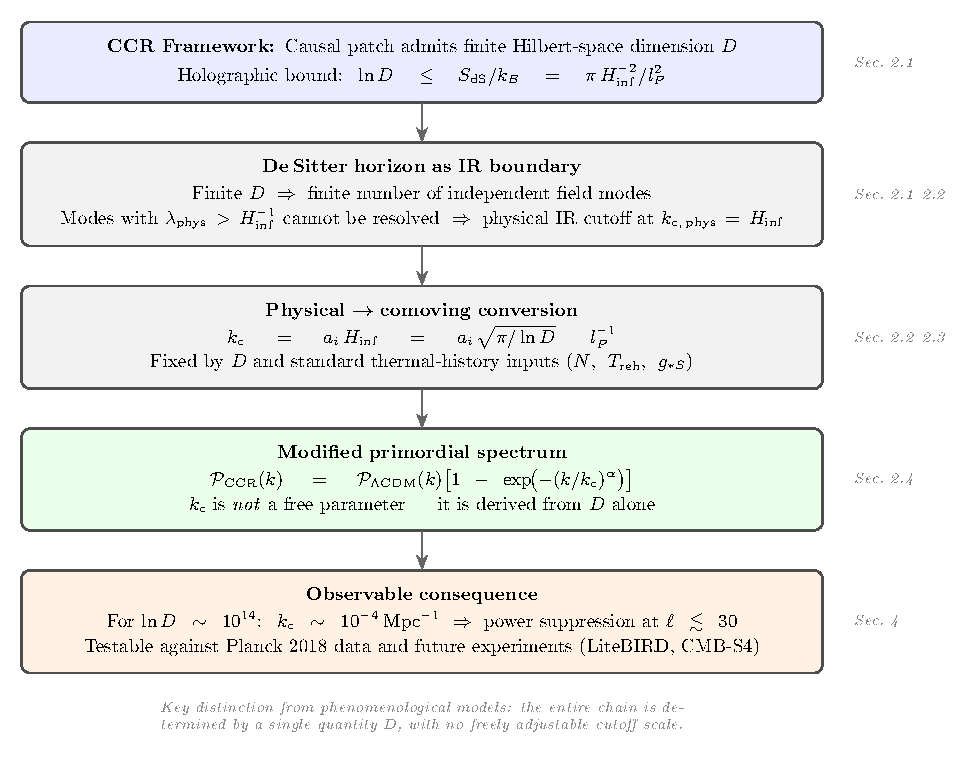
\includegraphics[width=\textwidth]{ccr_logical_chain}
  \caption{Logical chain from the CCR framework to the observable 
    CMB power suppression. The infrared cutoff $k_c$ is not a free 
    parameter but is uniquely determined by the Hilbert-space 
    dimension $D$ through the Gibbons--Hawking entropy bound.}
  \label{fig:logical_chain}
\end{figure}

In this section we obtain the infrared cutoff $k_c$ from the CCR framework
\cite{Chronis:2026}. The argument proceeds in three steps that each rest on
well-established physics: (i) during inflation the de~Sitter event horizon
defines the causal boundary of the patch, and the finite information capacity
of this patch---encoded in the Hilbert-space dimension $D$---truncates the
support of the quantum mode expansion at a physical scale set by $H_{\rm inf}$;
(ii) the CCR holographic bound uniquely relates $H_{\rm inf}$ to $D$; (iii)
converting to comoving wavenumbers via the inflationary expansion yields the
observable cutoff $k_c = k_c(D)$.
Unlike previous IR-cutoff models \cite{Contaldi:2003}, $k_c$ is not a free
parameter but a derived quantity, uniquely fixed by $D$.

% ------------------------------------------------------------
\subsection{The de~Sitter Horizon as a Natural IR Cutoff}
\label{subsec:dS_horizon}

During a quasi-de~Sitter inflationary epoch with Hubble parameter $H_{\rm inf}$,
the causal (event) horizon of a comoving observer is located at physical distance
%
\begin{equation}
  R_{\rm dS} \;=\; H_{\rm inf}^{-1} \;.
  \label{eq:RdS}
\end{equation}
%
In quantum field theory on de~Sitter space, the natural vacuum state is the
Bunch--Davies vacuum \cite{Bunch:1978}, in which sub-horizon modes
($k_{\rm phys} \gg H_{\rm inf}$) are well-described by Minkowski-space plane
waves, while super-horizon modes ($k_{\rm phys} \ll H_{\rm inf}$) freeze out
after horizon crossing and are subsequently stretched to cosmological scales
\cite{Mukhanov:2005,Birrell:1982,Baumann:2009,Ryden:2017}.
In the standard treatment with an infinite-dimensional Hilbert space, the mode
expansion extends to arbitrarily long wavelengths, and super-horizon modes are
set by initial conditions.

In the CCR framework, however, the Hilbert space of the causal patch has
\emph{finite} dimension $D$.
%
The consequences of this finiteness for the quantum field theory
within the patch can be stated precisely in effective-field-theory
(EFT) language.
%
A scalar field $\varphi$ in the Bunch--Davies vacuum, restricted to
a spatial volume $V \sim H_{\mathrm{inf}}^{-3}$, admits a discrete
set of mode functions $\{u_{\mathbf{k}}\}$ satisfying the
Klein--Gordon equation with appropriate boundary conditions.
%
In the standard treatment the mode sum extends over an infinite
tower of wavenumbers, each contributing an independent pair of
creation and annihilation operators $(\hat{a}_{\mathbf{k}},\,
\hat{a}_{\mathbf{k}}^\dagger)$ obeying the canonical commutation
relation $[\hat{a}_{\mathbf{k}},\,
\hat{a}_{\mathbf{k}'}^\dagger] = \delta_{\mathbf{k}\mathbf{k}'}$.
Each such pair spans a bosonic Fock space of unbounded dimension;
accommodating $\mathcal{N}$ independent modes therefore requires a
Hilbert space of dimension at least $d_{\min} \sim \mathcal{N}^p$,
where $p \geq 1$ depends on the occupancy truncation~\cite{Bousso:2000}.

The CCR constraint $\dim \mathcal{H} = D < \infty$ imposes an upper
bound on the number of independent mode pairs that can be faithfully
represented: the system admits at most $\mathcal{N}_{\max} \sim
(\ln D)^{1/p}$ independent degrees of freedom.
%
Modes with physical wavelength $\lambda_{\mathrm{phys}} >
H_{\mathrm{inf}}^{-1}$ would require additional degrees of freedom
beyond this budget; they are not dynamically excluded, but rather
\emph{have no independent state-space support} within the finite
Hilbert space of the patch.
%
This is an \emph{information-theoretic} truncation, analogous to the
UV cutoff that a lattice spacing imposes on a field theory---here
applied at the infrared end by the finite entropy capacity of the
de~Sitter horizon.

The horizon scale $H_{\mathrm{inf}}^{-1}$ therefore plays a dual
role: it is both the classical causal boundary and the IR resolution
limit of the finite-dimensional quantum theory.
%
We emphasise that this identification does not modify General
Relativity or the inflationary dynamics; it restricts only the
\emph{information content} of the quantum state accessible to a
single causal-patch observer.
%
The resulting effective IR cutoff is a \emph{controlled
approximation}: it is exact in the limit that the Gibbons--Hawking
entropy saturates the holographic bound (eq.~\eqref{eq:SdS}), and
it reduces smoothly to the standard infinite-dimensional treatment
in the limit $D \to \infty$.
The horizon-crossing condition
%
\begin{equation}
  k_{\rm phys} \;=\; H_{\rm inf}
  \label{eq:horizon_crossing}
\end{equation}
%
therefore defines the physical scale below which the finite-dimensional
Hilbert space can no longer support independent quantum fluctuations.
This identification is the central physical input of the CCR approach and
distinguishes it from both the standard infinite-dimensional treatment and
from ad hoc phenomenological cutoffs.

We note that the identification of the truncation scale with exactly $H_{\rm inf}$ 
is a simplifying assumption. In principle, the finite-dimensional mode budget 
could saturate at a scale $\beta H_{\rm inf}$ with $\beta = \mathcal{O}(1)$, 
which would shift $k_c \to \beta\, k_c$ throughout. Since $k_c$ enters 
logarithmically in the observable constraints (via $\ln D$), an 
$\mathcal{O}(1)$ prefactor does not qualitatively alter our results, but it 
does introduce a systematic uncertainty that should be addressed in a 
first-principles derivation of the mode truncation.

% ------------------------------------------------------------
\subsection{Connecting \texorpdfstring{$H_{\rm inf}$}{H\_inf} to the Hilbert-Space Dimension \texorpdfstring{$D$}{D}}
\label{subsec:H_to_D}

The CCR framework \cite{Chronis:2026} starts from assumption (A1): a causal
patch of area $A$ obeys the Bekenstein--Hawking entropy bound
\cite{Bekenstein:1973,Hawking:1975},
%
\begin{equation}
  S_{\max} \;\leq\; \frac{k_B\, A}{4\,l_P^2} \;,
  \label{eq:bekenstein}
\end{equation}
%
which implies a finite Hilbert-space dimension:
%
\begin{equation}
  \ln D \;\leq\; \frac{S_{\max}}{k_B} \;.
  \label{eq:lnD}
\end{equation}
%
For the de~Sitter patch with horizon radius $R_{\rm dS} = H_{\rm inf}^{-1}$,
the horizon area is $A = 4\pi R_{\rm dS}^2 = 4\pi H_{\rm inf}^{-2}$, and
the Gibbons--Hawking entropy \cite{Gibbons:1977} saturates the bound:
%
\begin{equation}
  S_{\rm dS} \;=\; \frac{k_B\,\pi}{H_{\rm inf}^2\,l_P^2} \;=\; \ln D \;.
  \label{eq:SdS}
\end{equation}
%
Solving for $H_{\rm inf}$:
%
\begin{equation}
  H_{\rm inf} \;=\; \frac{1}{l_P}\,\sqrt{\frac{\pi}{\ln D}} \;.
  \label{eq:H_inf}
\end{equation}
%
This is the key result: the Hubble parameter during inflation is uniquely
determined by the Hilbert-space dimension $D$ of the causal patch.
Combined with eq.~\eqref{eq:horizon_crossing}, the physical IR cutoff is
%
\begin{equation}
  k_{c,\,\rm phys} \;=\; H_{\rm inf} \;=\; \frac{1}{l_P}\,\sqrt{\frac{\pi}{\ln D}} \;.
  \label{eq:kc_phys}
\end{equation}
%
\paragraph{Physical interpretation.}
Equation~\eqref{eq:H_inf} states that a patch with a larger Hilbert-space
dimension $D$ (higher entropy capacity) corresponds to a \emph{lower}
inflationary Hubble rate, and hence a \emph{larger} causal horizon
$R_{\rm dS} = H_{\rm inf}^{-1}$.
A larger horizon admits longer-wavelength modes within the finite-dimensional
Hilbert space, so the IR cutoff $k_{c,\,\rm phys}$ shifts to smaller values
as $D$ increases.
In the limit $D \to \infty$ ($\ln D \to \infty$), $H_{\rm inf} \to 0$ and the
cutoff disappears: the Hilbert space becomes infinite-dimensional, the
information-theoretic truncation is removed, and the standard $\Lambda$CDM
power spectrum is recovered.
%
\paragraph{Saturation assumption.}
Equation~\eqref{eq:SdS} uses equality,
$\ln D = S_{\rm dS}/k_B$, corresponding to the assumption that the
de~Sitter entropy saturates the holographic bound.  If the bound is not
saturated, i.e.\ $\ln D = \xi\,S_{\rm dS}/k_B$ with $0 < \xi \leq 1$,
then $H_{\rm inf} \to H_{\rm inf}/\sqrt{\xi}$ and correspondingly
$k_c \to k_c/\sqrt{\xi}$: the cutoff shifts to \emph{larger} values,
producing \emph{stronger} suppression.  The saturated case $\xi = 1$
therefore yields the most conservative CCR prediction.  A detailed
discussion is given in appendix~\ref{app:derivation}.

% ------------------------------------------------------------
\subsection{From Physical to Comoving Wavenumber}
\label{subsec:comoving}

Observational CMB quantities are expressed in terms of \emph{comoving}
wavenumbers, which are constant during the expansion. The comoving IR cutoff
is obtained by multiplying the physical cutoff by the scale factor $a_i$ at the
onset of inflation (we normalise $a_0 = 1$ today):
%
\begin{equation}
  k_c \;=\; a_i\; k_{c,\,\rm phys} \;=\; \frac{a_i}{l_P}\,\sqrt{\frac{\pi}{\ln D}} \;.
  \label{eq:kc_comoving}
\end{equation}

% ---- CORRECTED a_i with entropy conservation ----
\paragraph{The scale factor $a_i$.}
Under the standard thermal history \cite{Kolb:1990,Ryden:2017}, the scale
factor at the onset of inflation is related to the present CMB temperature
$T_0$, the reheating temperature $T_{\rm reh}$, and the number of
inflationary e-folds $N$ through entropy conservation. The comoving entropy
density $s \propto g_{*S}\,T^3\,a^3$ is conserved after reheating, giving
%
\begin{equation}
  \frac{a_{\rm reh}}{a_0}
  \;=\;
  \left(\frac{g_{*S,0}}{g_{*S,\rm reh}}\right)^{\!1/3}
  \frac{T_0}{T_{\rm reh}} \;,
  \label{eq:entropy_conservation}
\end{equation}
%
where $g_{*S}$ denotes the effective number of relativistic degrees of freedom
contributing to entropy. Since $a_i = a_{\rm reh}\,e^{-N}$, we obtain
%
\begin{equation}
  a_i \;=\; e^{-N}
  \left(\frac{g_{*S,0}}{g_{*S,\rm reh}}\right)^{\!1/3}
  \frac{T_0}{T_{\rm reh}} \;.
  \label{eq:ai}
\end{equation}
%
We adopt $g_{*S,\rm reh} = 106.75$ (the full Standard Model value at
$T \gg 100\,\mathrm{GeV}$) and $g_{*S,0} = 3.938$ (photons plus three
neutrino species after $e^+e^-$ annihilation) \cite{Kolb:1990}, yielding
a correction factor
$(g_{*S,0}/g_{*S,\rm reh})^{1/3} \simeq 0.333$.
We fix the fiducial values $N = 60$ and $T_{\rm reh} = 10^{15}\,\mathrm{GeV}$,
consistent with standard slow-roll inflation and grand-unification-scale
reheating \cite{Baumann:2009}.

\paragraph{The key equation.}
Substituting eq.~\eqref{eq:ai} into eq.~\eqref{eq:kc_comoving}, the comoving
IR cutoff predicted by the CCR framework is
%
\begin{equation}
  \boxed{
    k_c \;=\; \frac{e^{-N}}{l_P}
    \left(\frac{g_{*S,0}}{g_{*S,\rm reh}}\right)^{\!1/3}
    \frac{T_0}{T_{\rm reh}}
    \sqrt{\frac{\pi}{\ln D}}
  }
  \label{eq:kc_final}
\end{equation}
%
This is the central result of this section. $k_c$ is \emph{not} a free
parameter: it is a derived function of the single fundamental quantity $D$,
given fixed thermal-history parameters.
For the fiducial values above and $T_0 = 2.7255\,\mathrm{K}$:
%
\begin{equation}
  k_c \;\simeq\; 1.6\times 10^{-4}\,\mathrm{Mpc}^{-1}
  \qquad\text{for}\quad \ln D \;\simeq\; 2.0\times 10^{14} \;.
  \label{eq:kc_numerical}
\end{equation}
%
This value lies within the observable window
($k_c \sim 10^{-4}$--$10^{-3}\,\mathrm{Mpc}^{-1}$) relevant for low-$\ell$
CMB suppression. The corresponding inflationary Hubble rate is
$H_{\rm inf} \simeq 1.5\times 10^{12}\,\mathrm{GeV}$, a factor $\sim 40$
below the observational upper bound
$H_{\rm inf} < 6\times 10^{13}\,\mathrm{GeV}$ set by Planck tensor-mode
constraints \cite{Planck:2018inflation}.

Table~\ref{tab:derived_quantities} lists the derived CCR quantities for a
range of $\ln D$ values, demonstrating the smooth dependence of $k_c$ on
the Hilbert-space dimension.

\begin{table}[t]
  \centering
  \begin{tabular}{ccccc}
    \hline\hline
    $\ln D$ & $k_c$ [Mpc$^{-1}$] & $H_{\rm inf}$ [GeV]
      & $R_{\rm dS}$ [m] & $R_{\rm dS}$ [$l_P$] \\
    \hline
    $1.0\times 10^{13}$ & $7.33\times 10^{-4}$ & $6.84\times 10^{12}$
      & $2.88\times 10^{-29}$ & $1.78\times 10^{6}$ \\
    $5.0\times 10^{13}$ & $3.28\times 10^{-4}$ & $3.06\times 10^{12}$
      & $6.45\times 10^{-29}$ & $3.99\times 10^{6}$ \\
    $1.0\times 10^{14}$ & $2.32\times 10^{-4}$ & $2.16\times 10^{12}$
      & $9.12\times 10^{-29}$ & $5.64\times 10^{6}$ \\
    $2.0\times 10^{14}$ & $1.64\times 10^{-4}$ & $1.53\times 10^{12}$
      & $1.29\times 10^{-28}$ & $7.98\times 10^{6}$ \\
    $5.0\times 10^{14}$ & $1.04\times 10^{-4}$ & $9.68\times 10^{11}$
      & $2.04\times 10^{-28}$ & $1.26\times 10^{7}$ \\
    $1.0\times 10^{15}$ & $7.33\times 10^{-5}$ & $6.84\times 10^{11}$
      & $2.88\times 10^{-28}$ & $1.78\times 10^{7}$ \\
    \hline\hline
  \end{tabular}
  \caption{Derived CCR quantities for fiducial parameters $N = 60$,
    $T_{\rm reh} = 10^{15}\,\mathrm{GeV}$,
    $g_{*S,\rm reh} = 106.75$, $g_{*S,0} = 3.938$.
    The Contaldi et al.\ \cite{Contaldi:2003} best-fit value
    $k_c \simeq 4.9\times 10^{-4}\,\mathrm{Mpc}^{-1}$ corresponds to
    $\ln D \simeq 2.2\times 10^{13}$ in the CCR framework.
    All values of $H_{\rm inf}$ lie well below the Planck tensor-mode
    upper bound $H_{\rm inf} < 6\times 10^{13}\,\mathrm{GeV}$.}
  \label{tab:derived_quantities}
\end{table}

% ------------------------------------------------------------
\subsection{The Just-Enough-Inflation Condition}
\label{subsec:just_enough}

For $k_c$ to produce an observable suppression in the Planck low-$\ell$ data,
it must be comparable to the present Hubble scale
$a_0 H_0 \simeq 2.3\times 10^{-4}\,h\,\mathrm{Mpc}^{-1}$.
From eq.~\eqref{eq:kc_final}, this requires $N \approx 60$ e-folds of
inflation, precisely the minimum needed to solve the horizon and flatness
problems~\cite{Baumann:2009}: the \emph{just-enough-inflation} condition.
If $N \gg 60$, the comoving cutoff is redshifted beyond the observable
universe; if $N \ll 60$, it moves to $\ell > 30$, conflicting with the
acoustic-peak structure.

The observability of $k_c$ for $N \approx 60$ does not require an
exponentially narrow range of $e$-folds; it occupies a non-negligible
fraction of the physically motivated $N$ range, as quantified below.

% ---- NEW: Quantitative fine-tuning assessment ----
\paragraph{Quantitative assessment.}
To quantify the sensitivity of $k_c$ to $N$, we define the observable window
as $k_c \in [10^{-4},\, 2\times 10^{-3}]\,\mathrm{Mpc}^{-1}$, corresponding
to suppression at multipoles $\ell \lesssim 30$.
For the fiducial values $\ln D = 2\times 10^{14}$ and
$T_{\rm reh} = 10^{15}\,\mathrm{GeV}$, this window is satisfied for
$N \in [57.5,\, 60.5]$, a range of $\Delta N \simeq 3$ e-folds
(see figure~\ref{fig:N_bandwidth}).
Since the horizon and flatness problems independently require $N \gtrsim 55$,
the observable range of $k_c$ occupies a finite fraction
($\Delta N / N \sim 5\%$) of the physically motivated
$N$ range, rather than demanding a precise value.

Conversely, for $\sim 95\%$ of the physically motivated $N$ range the cutoff 
is redshifted beyond the observable window, so the default expectation is that 
the CCR suppression is undetectable. Observability therefore requires a 
moderate coincidence between the duration of inflation and the horizon scale 
--- a point we regard as a quantitative fine-tuning caveat rather than a 
fundamental obstacle, but one that should be borne in mind when interpreting 
any future detection.

\begin{figure}[t]
  \centering
  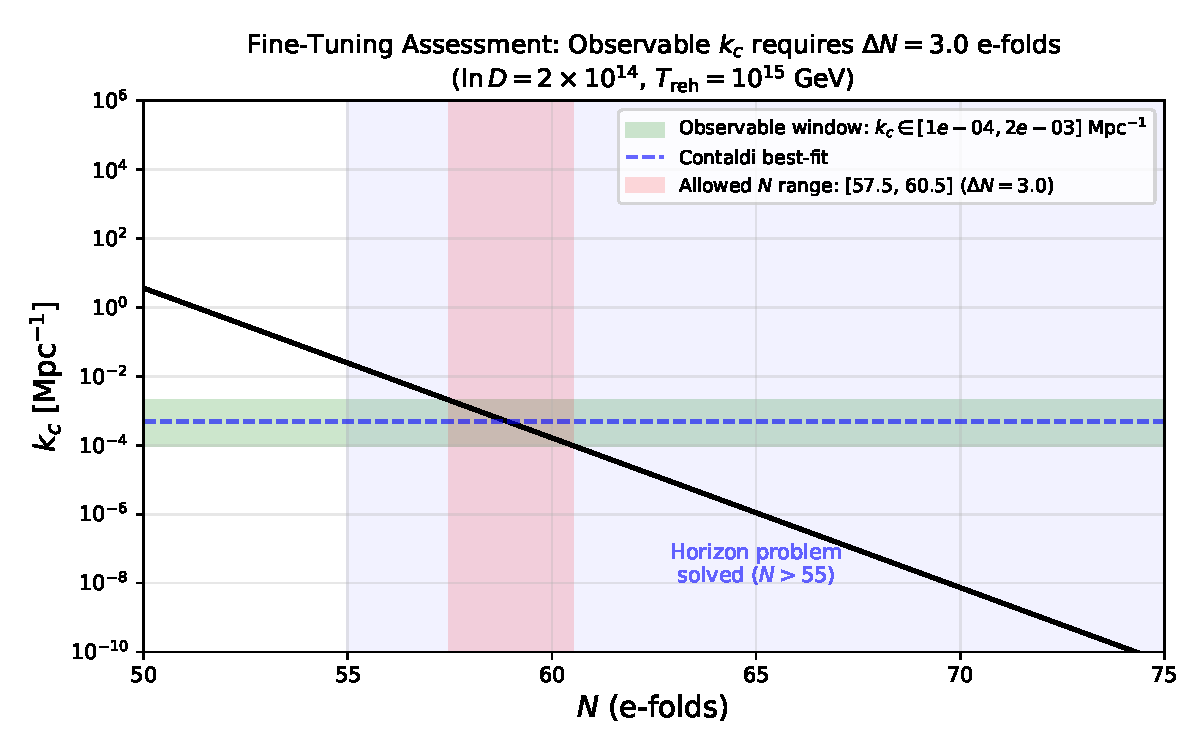
\includegraphics[width=0.65\linewidth]{N_bandwidth}
  \caption{Observable bandwidth in $N$. The shaded region marks
    $N \in [57.5,\,60.5]$ for which $k_c$ falls in the observable window
    $k_c \in [10^{-4},\,2\times 10^{-3}]\,\mathrm{Mpc}^{-1}$, at fixed
    $\ln D = 2\times 10^{14}$ and $T_{\rm reh} = 10^{15}\,\mathrm{GeV}$.
    Horizontal dashed lines mark the observable-window boundaries.
    The range $\Delta N \simeq 3$ represents $\sim 5\%$ of the
    physically motivated $N \in [55,70]$ prior.}
  \label{fig:N_bandwidth}
\end{figure}

% ---- NEW: Sensitivity analysis paragraph ----
\paragraph{Degeneracy and sensitivity to thermal-history parameters.}
Equation~\eqref{eq:kc_final} shows that $k_c$ depends on $N$, $T_{\rm reh}$,
and $g_{*S}$ in addition to $D$, introducing degeneracies in the
$(D,\,N,\,T_{\rm reh})$ parameter space.
In this work we break these degeneracies by fixing $N = 60$ and
$T_{\rm reh} = 10^{15}\,\mathrm{GeV}$, reducing $k_c$ to a function of $D$
alone. We have verified that the results are robust under variations of $N$
and $T_{\rm reh}$ within physically motivated ranges:
table~\ref{tab:sensitivity} presents $k_c$ for
$N \in [50,70]$ and $T_{\rm reh} \in [10^{10}, 10^{16}]\,\mathrm{GeV}$
at fixed $\ln D = 2\times 10^{14}$.
The observable window $k_c \sim 10^{-4}$--$10^{-3}\,\mathrm{Mpc}^{-1}$
is achieved for a broad range of $(N,\,T_{\rm reh})$ combinations
(see figure~\ref{fig:kc_contour}).
A full marginalisation over $N$ and $T_{\rm reh}$ with physically motivated
priors is a natural extension of this analysis, but is beyond the scope of
the present phenomenological study.

\begin{table}[t]
  \centering
  \caption{Sensitivity of $k_c$ [Mpc$^{-1}$] to the number of e-folds $N$
    and reheating temperature $T_{\rm reh}$, for fixed
    $\ln D = 2\times 10^{14}$.
    The observable window
    $k_c \sim 10^{-4}$--$10^{-3}\,\mathrm{Mpc}^{-1}$ is highlighted.}
  \label{tab:sensitivity}
  \begin{tabular}{cccccc}
    \hline\hline
    $N$ & $10^{10}$ GeV & $10^{12}$ GeV & $10^{14}$ GeV
        & $10^{15}$ GeV & $10^{16}$ GeV \\
    \hline
    50 & $3.6\times 10^{5}$ & $3.6\times 10^{3}$ & $3.6\times 10^{1}$
       & $3.6\times 10^{0}$ & $3.6\times 10^{-1}$ \\
    55 & $2.4\times 10^{3}$ & $2.4\times 10^{1}$ & $2.4\times 10^{-1}$
       & $2.4\times 10^{-2}$ & $2.4\times 10^{-3}$ \\
    60 & $1.6\times 10^{1}$ & $1.6\times 10^{-1}$ & $\mathbf{1.6\times 10^{-3}}$
       & $\mathbf{1.6\times 10^{-4}}$ & $1.6\times 10^{-5}$ \\
    65 & $1.1\times 10^{-1}$ & $1.1\times 10^{-3}$ & $1.1\times 10^{-5}$
       & $1.1\times 10^{-6}$ & $1.1\times 10^{-7}$ \\
    70 & $7.4\times 10^{-4}$ & $7.4\times 10^{-6}$ & $7.4\times 10^{-8}$
       & $7.4\times 10^{-9}$ & $7.4\times 10^{-10}$ \\
    \hline\hline
  \end{tabular}
\end{table}

\begin{figure}[t]
  \centering
  \begin{minipage}{0.48\linewidth}
    \centering
    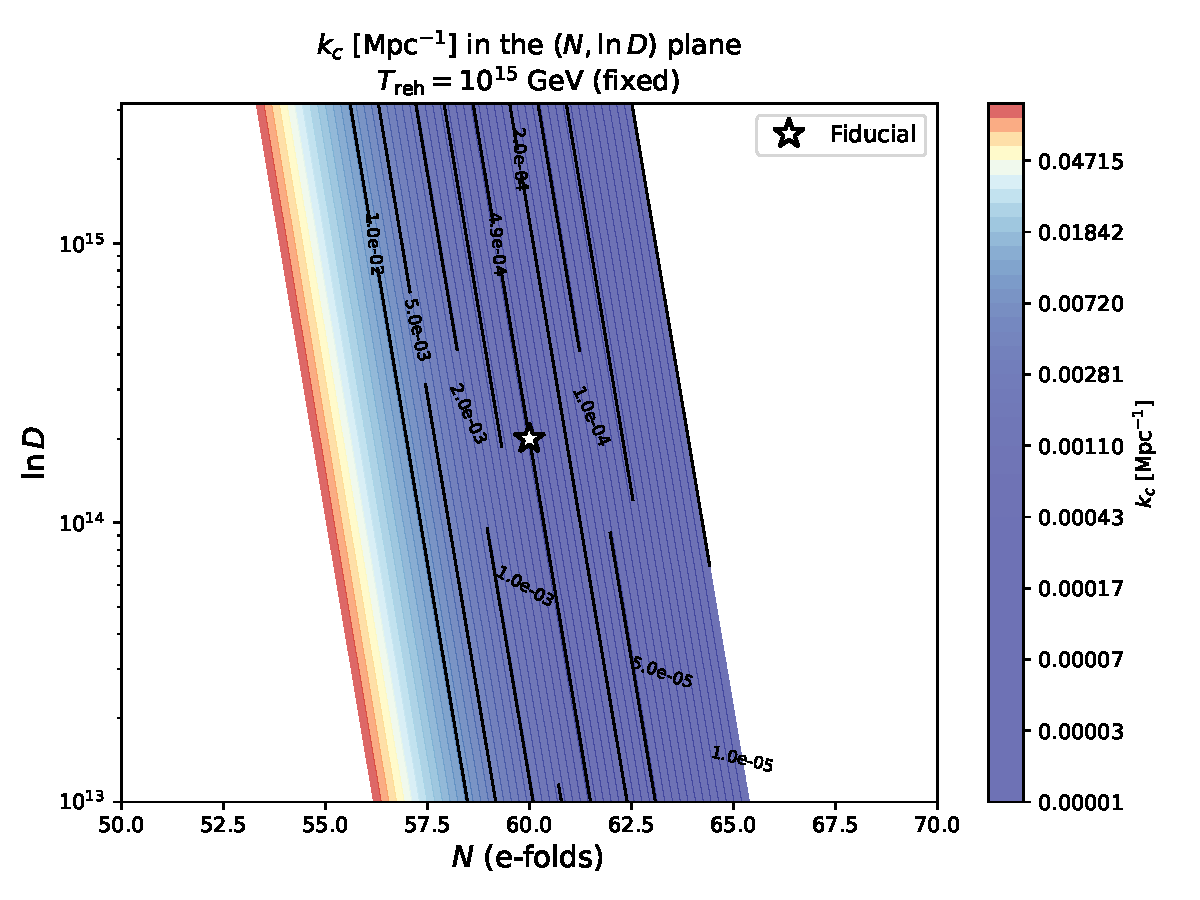
\includegraphics[width=\linewidth]{kc_contour_N_lnD}
  \end{minipage}
  \hfill
  \begin{minipage}{0.48\linewidth}
    \centering
    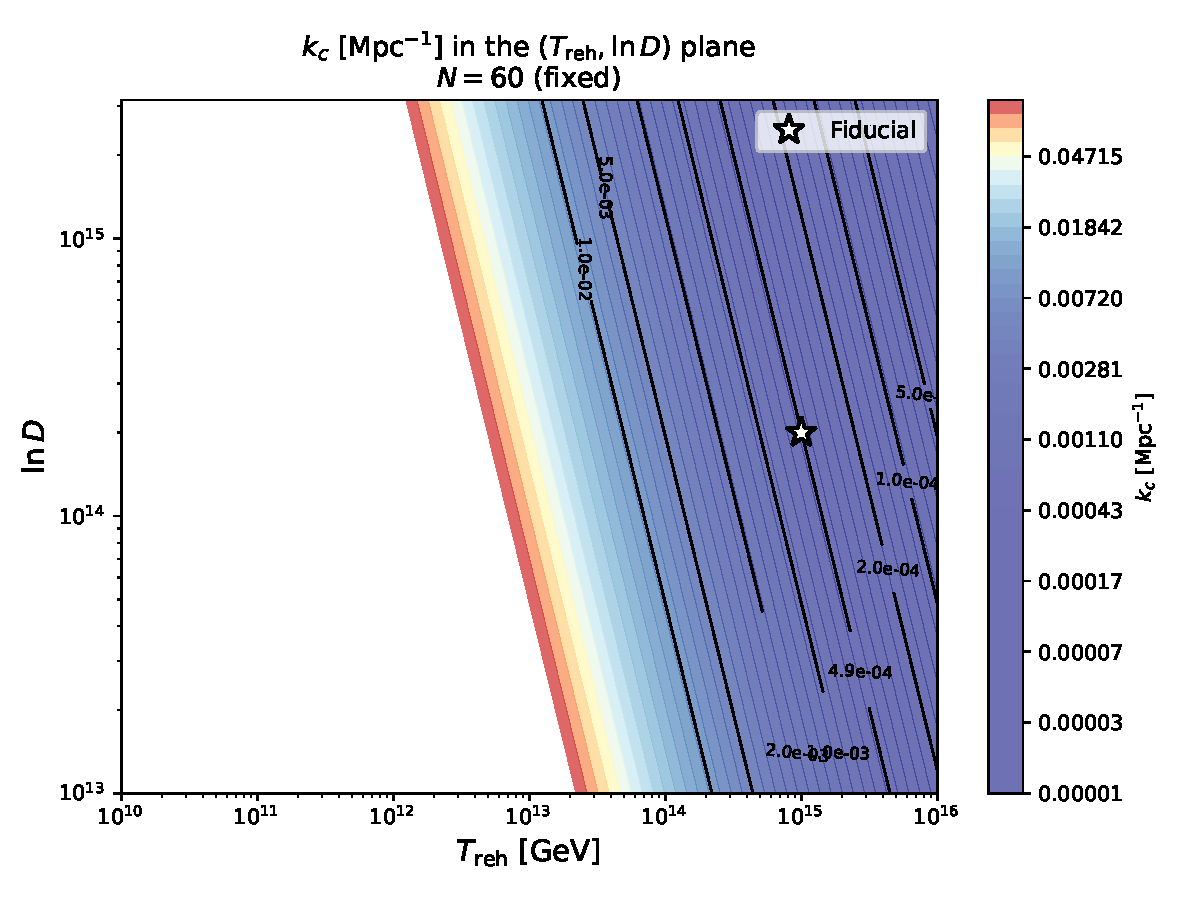
\includegraphics[width=\linewidth]{kc_contour_Treh_lnD}
  \end{minipage}
  \caption{Contour plots of $k_c$ [$\mathrm{Mpc}^{-1}$] in the
    $(N,\,\ln D)$ plane (\textit{left}) and the
    $(T_{\rm reh},\,\ln D)$ plane (\textit{right}).
    The green band marks the observable window
    $k_c \in [10^{-4},\,10^{-3}]\,\mathrm{Mpc}^{-1}$.
    The right panel is evaluated at fixed $N = 60$;
    the left panel at fixed $T_{\rm reh} = 10^{15}\,\mathrm{GeV}$.}
  \label{fig:kc_contour}
\end{figure}

% ------------------------------------------------------------
\subsection{The CCR-Modified Primordial Power Spectrum}
\label{subsec:power_spectrum}

The finite Hilbert-space dimension $D$ suppresses primordial fluctuations at
$k < k_c$: the finite information capacity of the causal patch truncates the
mode expansion, so that modes with wavelengths exceeding $H_{\rm inf}^{-1}$
have no independent degrees of freedom in which to carry quantum fluctuations.
We model this suppression as:
%
\begin{equation}
  \mathcal{P}_{\rm CCR}(k) \;=\; A_s
  \left(\frac{k}{k_*}\right)^{n_s-1}
  \left[1 - \exp\!\left(-\left(\frac{k}{k_c}\right)^{\!\alpha}\right)\right] ,
  \label{eq:P_CCR}
\end{equation}
%
where $A_s$ is the scalar amplitude, $k_* = 0.05\,\mathrm{Mpc}^{-1}$ is the
pivot scale, $n_s$ is the scalar spectral index, and $\alpha > 0$ controls
the sharpness of the transition.

\paragraph{Limiting behaviour.}
For $k \gg k_c$ the exponential vanishes and the standard Harrison--Zel'dovich
spectrum is recovered. For $D \to \infty$ (equivalently $k_c \to 0$), the full
$\Lambda$CDM power spectrum is recovered at all scales, confirming that the
CCR-modified spectrum is a one-parameter deformation of the standard model
with a well-defined limit. We have verified this recovery numerically
(see section~\ref{sec:results}).

% ---- REVISED: alpha justification ----
\paragraph{The shape parameter $\alpha$.}
The CCR framework predicts the existence of the cutoff scale $k_c$ but does
not uniquely fix the shape of the transition in this phenomenological treatment.
The shape depends on the detailed microphysics of mode generation at horizon
crossing. 
Preliminary numerical solutions of the Mukhanov--Sasaki equation in a truncated 
mode space suggest $\alpha \in [2, 3]$ depending on
the boundary prescription (Dirichlet, Neumann, or Danielsson
vacuum), consistent with the posterior range obtained in this
analysis; a detailed derivation will be presented separately.
At the level of phenomenological template behaviour, different
values of $\alpha$ produce qualitatively distinct suppression profiles:
$\alpha = 1$ gives a gradual exponential suppression;
$\alpha = 2$ produces a Gaussian-like cutoff; larger values
$\alpha \gtrsim 4$ approach a sharp step function.

We treat $\alpha$ as a free parameter with flat prior $\alpha \in [1,6]$.
The lower bound ensures a smooth, physically motivated transition,
while the upper bound avoids numerical artefacts in the CAMB Boltzmann
integration (see section~\ref{sec:methodology}).
Figure~\ref{fig:suppression_alpha} shows the suppression factor
$\mathcal{P}_{\rm CCR}/\mathcal{P}_{\Lambda\rm CDM}$ for several values of
$\alpha$: the curves differ appreciably within the $\ell = 2$--$30$
wavenumber range, indicating that CMB data can discriminate between different
transition shapes.

\begin{figure}[t]
  \centering
  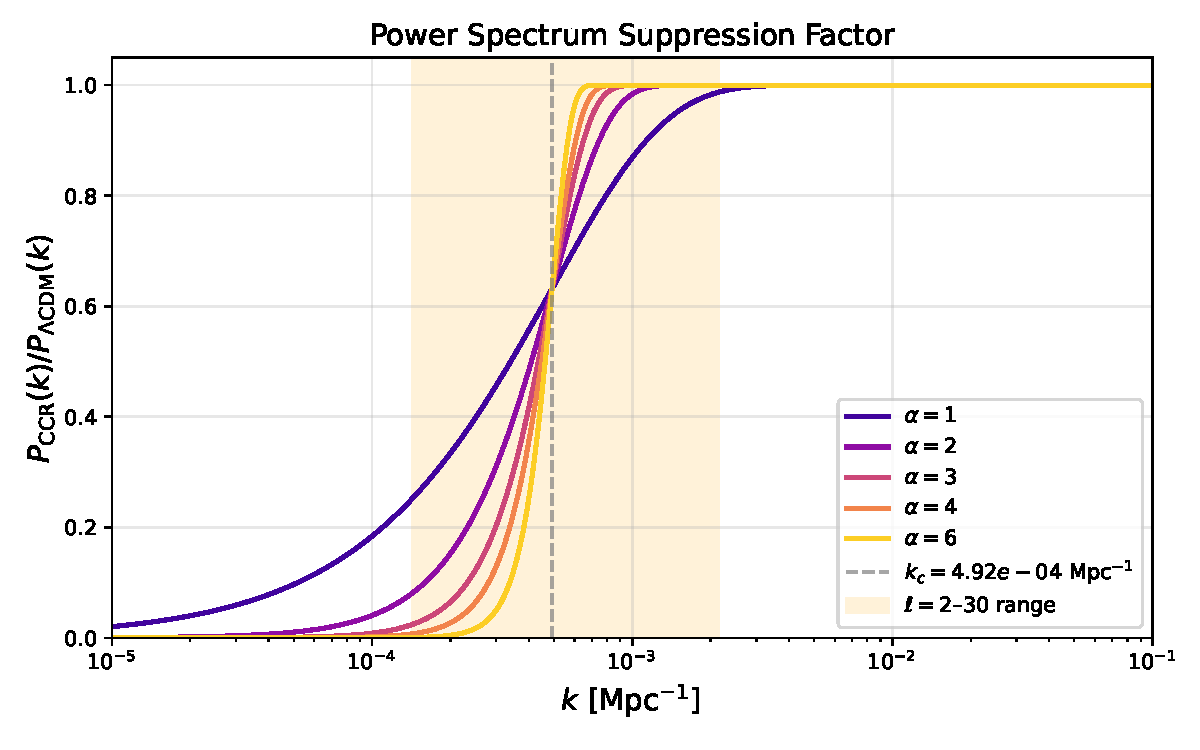
\includegraphics[width=0.65\linewidth]{suppression_factor_alpha}
  \caption{Suppression factor
    $\mathcal{P}_{\rm CCR}(k)/\mathcal{P}_{\Lambda\rm CDM}(k)$
    as a function of $k/k_c$ for shape parameters
    $\alpha = 1,\,2,\,3,\,4,\,6$ (see eq.~\eqref{eq:P_CCR}).
    Larger $\alpha$ produces a sharper transition; $\alpha = 1$ gives
    a gradual exponential suppression.
    All curves are evaluated at the fiducial cutoff
    $k_c = 1.6\times 10^{-4}\,\mathrm{Mpc}^{-1}$.}
  \label{fig:suppression_alpha}
\end{figure}

\paragraph{Remark on the parameter count.}
It is important to distinguish between the number of \emph{sampled}
parameters and the number of \emph{free} parameters.  The CCR model
samples two parameters beyond $\Lambda$CDM: $\log_{10}(\ln D)$ and
$\alpha$.  However, $k_c$ is not independently free---it is a
deterministic function of $\ln D$ via eq.~(\ref{eq:kc_comoving}).
In contrast, the Contaldi et al.\ model treats both $k_c$ and
$\alpha$ as independent free parameters.  The CCR framework therefore
replaces one phenomenological degree of freedom ($k_c$) with a
theoretically motivated one ($\ln D$), while simultaneously
generating a prediction for the tensor-to-scalar ratio
(section~\ref{subsec:tensor_ratio}) that is absent from the purely
phenomenological approach.  The shape parameter $\alpha$ remains free
because it encodes the microphysics of the cutoff transition, which
the CCR framework does not determine at this level.  A first-principles
derivation of $\alpha$ from the Mukhanov--Sasaki equation in a
finite-dimensional Hilbert space is the natural next step, but lies
beyond the scope of this work.

% ------------------------------------------------------------
\subsection{Comparison with Contaldi et al.\ (2003)}
\label{subsec:contaldi}

The functional form of eq.~\eqref{eq:P_CCR} is formally identical to the
exponential-cutoff template of ref.~\cite{Contaldi:2003}. The two approaches
differ, however, in a fundamental respect summarised in
table~\ref{tab:comparison}.

In ref.~\cite{Contaldi:2003}, $k_c$ is a free phenomenological parameter
introduced to improve the fit to low-$\ell$ data, with physical motivation
limited to a model-specific kinetic-domination stage before slow-roll
inflation. There is no connection to an independently published theoretical
framework, and no prediction for any other observable.

In this work, $k_c$ is entirely determined by $D$ through
eq.~\eqref{eq:kc_final}. The CCR framework \cite{Chronis:2026} provides an
independently peer-reviewed foundation: the finite information capacity of
the de~Sitter patch sets $H_{\rm inf}$ via the Gibbons--Hawking entropy,
and $H_{\rm inf}$ is the natural IR cutoff of the Bunch--Davies spectrum.
The sampled parameter is $D$; $k_c$ follows deterministically.
This connection between the quantum information content of the
de~Sitter patch and the CMB power spectrum is the distinguishing
feature of the present analysis relative to purely phenomenological
cutoff models.

\begin{table}[t]
  \centering
  \begin{tabular}{lcc}
    \hline\hline
    & \textbf{Contaldi et al.\ (2003)} & \textbf{This work (CCR)} \\
    \hline
    IR cutoff origin    & Kinetic domination (ad hoc) & De~Sitter horizon $H_{\rm inf}$ \\
    $H_{\rm inf}$ determined by & Not addressed & $\ln D$ via Gibbons--Hawking \\
    Sampled parameter   & $k_c$ (free)  & $D$ (fundamental) \\
    $k_c$ status        & Free parameter & Derived: $k_c = k_c(D)$ \\
    Independent framework & No           & Yes (CCR, \cite{Chronis:2026}) \\
    $\alpha$ treatment  & Fixed (3.35)  & Free, $\alpha\in[1,6]$ \\
    Entropy correction  & Not applicable & $g_{*S}$ included \\
    Observational constraints on & $k_c$ & $D$ and $H_{\rm inf}$ \\
    \hline\hline
  \end{tabular}
  \caption{Comparison between the Contaldi et al.\ \cite{Contaldi:2003}
    phenomenological IR cutoff and the CCR-motivated cutoff of this work.
    The key distinction is that $k_c$ is a free parameter in the former
    and a derived quantity in the latter.}
  \label{tab:comparison}
\end{table}


% ============================================================
% Section 2.7: Tensor-to-Scalar Ratio Prediction
% Insert after Section 2.6 (Comparison with Contaldi et al.)
% ============================================================

\subsection{Prediction for the Tensor-to-Scalar Ratio}
\label{subsec:tensor_ratio}

The CCR framework determines $H_{\rm inf}$ from $D$ via eq.~\eqref{eq:H_inf},
which yields a direct prediction for the tensor-to-scalar ratio $r$.
The tensor power spectrum amplitude at horizon crossing is
\begin{equation}
  \mathcal{P}_T = \frac{2}{\pi^2}\,\frac{H_{\rm inf}^2}{M_{\rm Pl}^2}\,,
  \label{eq:tensor_spectrum}
\end{equation}
where $M_{\rm Pl} = (8\pi G)^{-1/2} \simeq 2.435\times 10^{18}\,\mathrm{GeV}$
is the reduced Planck mass. Since $M_{\rm Pl} = m_{\rm Pl}/\sqrt{8\pi}$ and
$H_{\rm inf} = m_{\rm Pl}\sqrt{\pi/\ln D}$ from eq.~\eqref{eq:H_inf},
\begin{equation}
  \frac{H_{\rm inf}}{M_{\rm Pl}} = \sqrt{\frac{8\pi^2}{\ln D}}\,.
\end{equation}
The tensor-to-scalar ratio is then
\begin{equation}
  r \;=\; \frac{\mathcal{P}_T}{A_s}
    \;=\; \frac{2}{\pi^2 A_s}\,\frac{H_{\rm inf}^2}{M_{\rm Pl}^2}
    \;=\; \frac{16}{A_s\,\ln D}\,.
  \label{eq:r_CCR}
\end{equation}
This is a parameter-free prediction: given the observed scalar amplitude
$A_s \simeq 2.1\times 10^{-9}$ and a value of $\ln D$, the tensor-to-scalar
ratio is uniquely determined. For the fiducial value $\ln D = 2\times 10^{14}$,
\begin{equation}
  r \;\simeq\; 3.8\times 10^{-5}\,,
\end{equation}
which is a factor $\sim 1500$ below the current observational upper bound
$r_{0.002} < 0.056$ (95\% CL) from Planck+BK15~\cite{Planck:2018inflation},
and a factor $\sim 1000$ below the current best constraint
$r < 0.034$ (95\% CL) from the combination of Planck,
SPT, ACT, and BICEP/Keck data~\cite{Campeti:2025}

Table~\ref{tab:tensor_ratio} lists the predicted $r$ for a range of $\ln D$ values.
The current tensor-mode bounds impose only a weak lower bound on the Hilbert
space dimension, $\ln D \gtrsim 2\times 10^{11}$, which is far below the regime
probed by the low-$\ell$ power spectrum suppression. More stringent constraints
require future experiments: the predicted $r$ enters the sensitivity window
of LiteBIRD~\cite{LiteBIRD:2022} ($r \sim 10^{-3}$) only for
$\ln D \lesssim 8\times 10^{12}$, at the lower edge of our prior range.

\begin{table}[t]
  \centering
  \begin{tabular}{ccc}
    \hline\hline
    $\ln D$ & $r$ & Status \\
    \hline
    $1.0\times 10^{12}$ & $7.6\times 10^{-3}$ & Detectable by LiteBIRD \\
    $1.0\times 10^{13}$ & $7.6\times 10^{-4}$ & Below LiteBIRD sensitivity \\
    $5.0\times 10^{13}$ & $1.5\times 10^{-4}$ & Below LiteBIRD sensitivity \\
    $1.0\times 10^{14}$ & $7.6\times 10^{-5}$ & Below LiteBIRD sensitivity \\
    $\mathbf{2.0\times 10^{14}}$ & $\mathbf{3.8\times 10^{-5}}$ & Below LiteBIRD sensitivity \\
    $1.0\times 10^{15}$ & $7.6\times 10^{-6}$ & Below LiteBIRD sensitivity \\
    $1.0\times 10^{16}$ & $7.6\times 10^{-7}$ & Below LiteBIRD sensitivity \\
    \hline\hline
  \end{tabular}
  \caption{CCR prediction for the tensor-to-scalar ratio $r = 16/(A_s\,\ln D)$,
    with $A_s = 2.1\times 10^{-9}$. The fiducial value is shown in bold.
    Current bounds ($r < 0.056$ from Planck+BK15, $r < 0.036$ from BICEP/Keck,
    $r < 0.034$ from the combined CMB analysis of ref.~\cite{Campeti:2025})
    are satisfied for the entire prior range $\ln D \in [10^{12}, 10^{16}]$.
    LiteBIRD sensitivity ($r \sim 10^{-3}$) probes only the lowest end of
    the $\ln D$ range.}
  \label{tab:tensor_ratio}
\end{table}

\paragraph{Physical interpretation.}
The inverse relation $r \propto 1/\ln D$ has a transparent physical origin:
a larger Hilbert space dimension $D$ corresponds to a lower inflationary
energy scale $H_{\rm inf}$ (eq.~\eqref{eq:H_inf}), which in turn produces
a smaller tensor amplitude. The CCR framework thus generically predicts
\emph{small} $r$, consistent with the non-detection of primordial
gravitational waves by all experiments to date. This is in contrast to
large-field inflation models (e.g., $V \propto \phi^2$) that predict $r \sim 0.1$
and are increasingly disfavoured by the data~\cite{Planck:2018inflation}.

\paragraph{Complementarity with the IR cutoff.}
Equations~\eqref{eq:kc_final} and~\eqref{eq:r_CCR} provide two
independent observational signatures of $\ln D$: the infrared cutoff
$k_c$ probed by the low-$\ell$ TT spectrum, and the tensor-to-scalar
ratio $r$ probed by B-mode polarisation. Any future joint constraint
on $(k_c, r)$ therefore provides a powerful consistency test of the CCR
framework, since both quantities are deterministic functions of the
single parameter $\ln D$ (at fixed thermal history). In particular,
a detection of $r \gtrsim 10^{-3}$ would imply $\ln D \lesssim 10^{13}$,
which in turn predicts $k_c \gtrsim 7\times 10^{-4}\,\mathrm{Mpc}^{-1}$
--- a strong, potentially measurable suppression in the low-$\ell$ power
spectrum. Conversely, the absence of low-$\ell$ suppression at the level
predicted for $\ln D \lesssim 10^{13}$ would rule out the parameter space
accessible to tensor-mode experiments.

Figure~\ref{fig:tensor_ratio} shows the CCR prediction for $r$ as a function
of $\ln D$, together with current and projected observational bounds.

\begin{figure}[t]
  \centering
  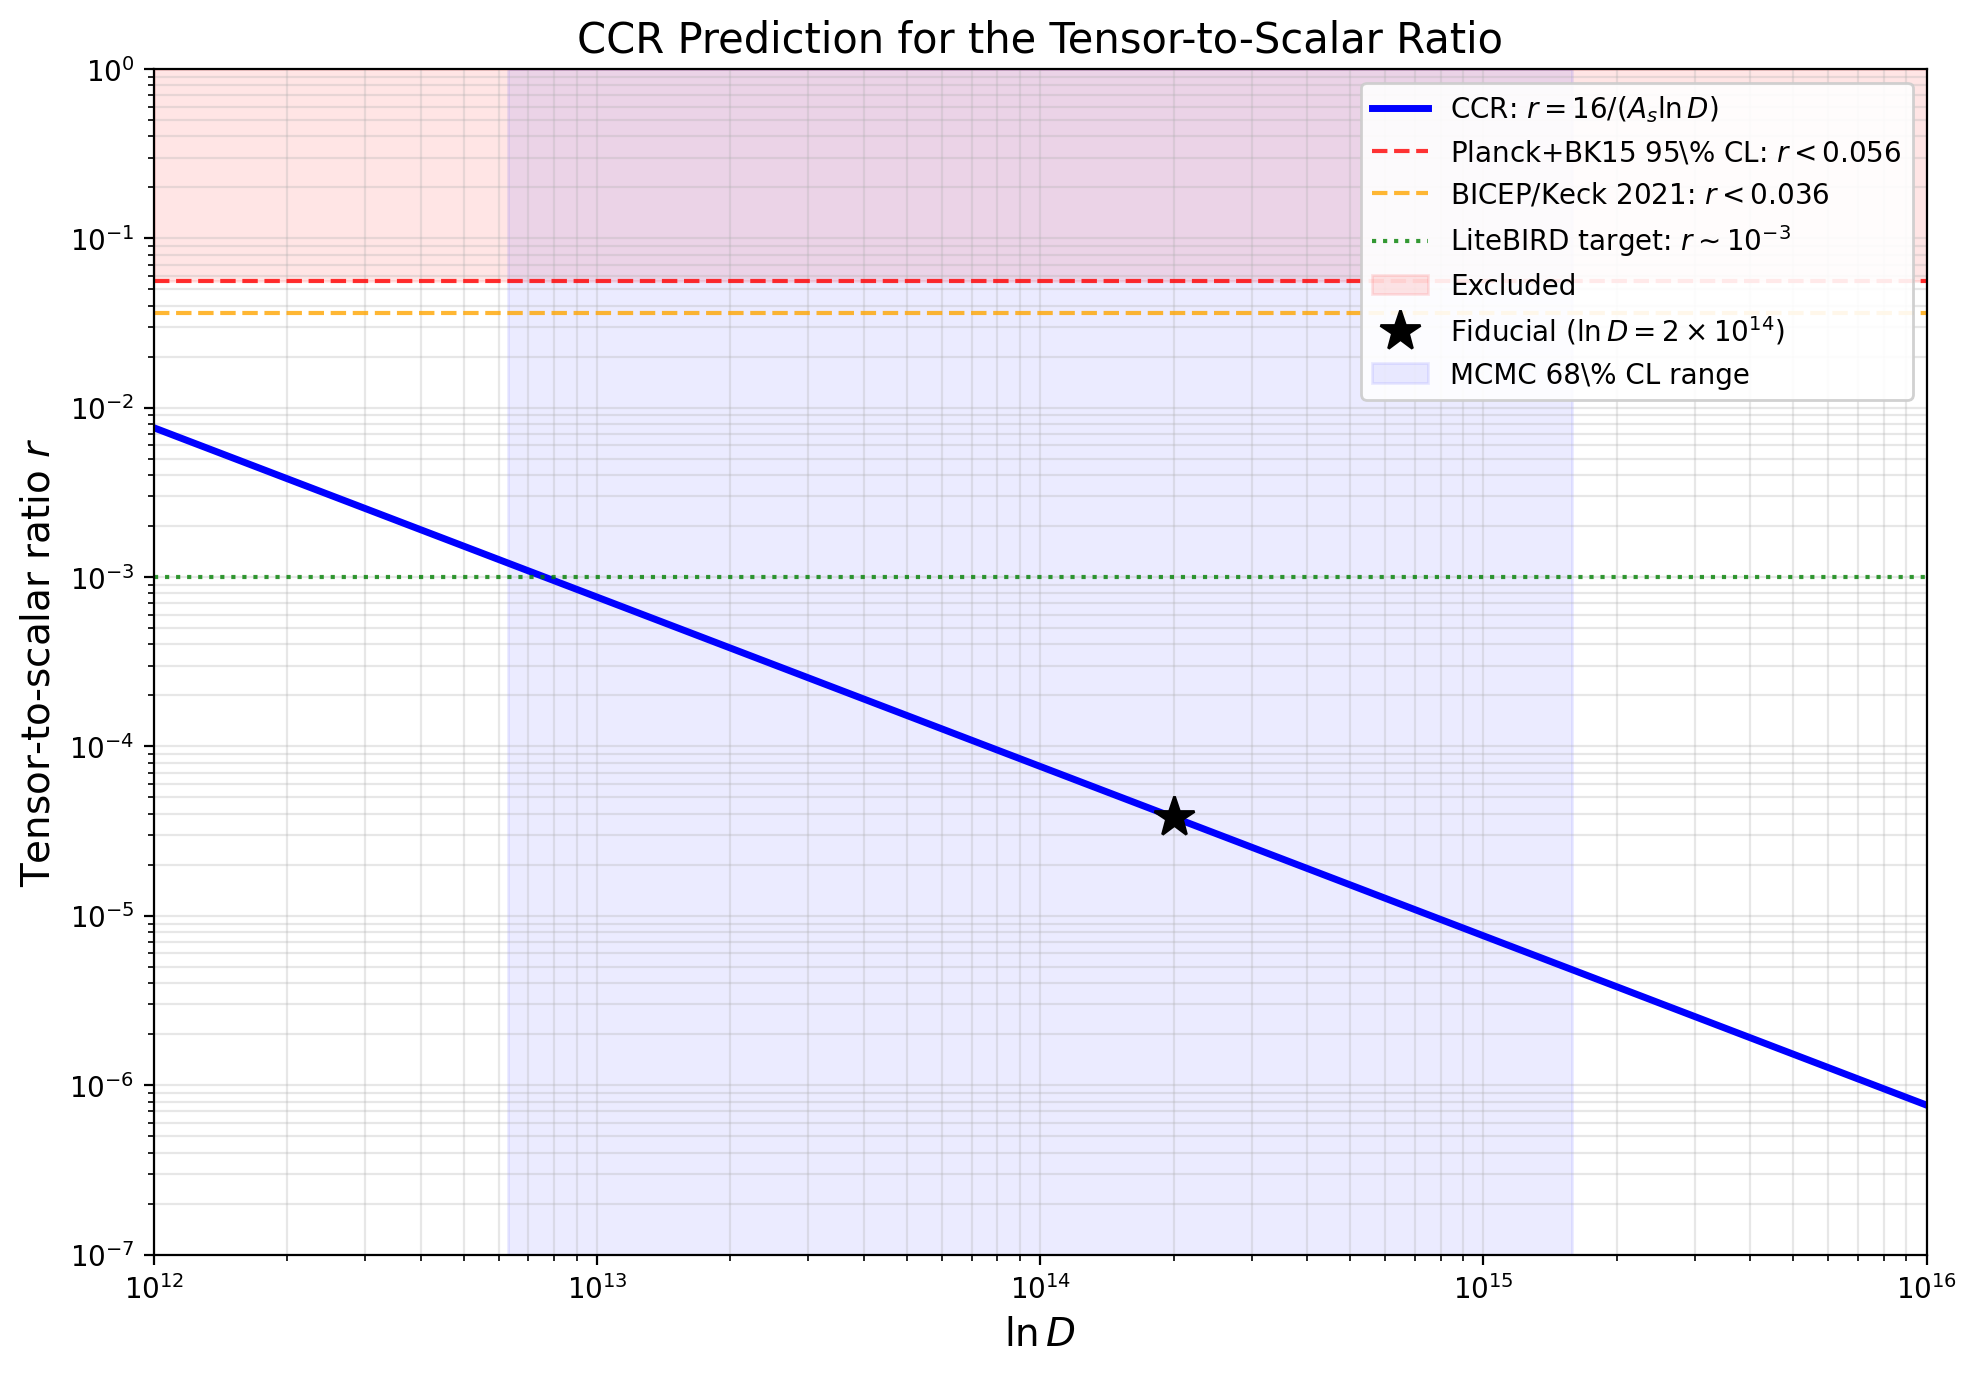
\includegraphics[width=0.75\linewidth]{tensor_ratio_prediction}
  \caption{CCR prediction for the tensor-to-scalar ratio $r$ as a function of
    $\ln D$ (solid blue line), compared with current observational upper limits
    (Planck+BK15 95\% CL: $r < 0.056$; BICEP/Keck 2021: $r < 0.036$;
    combined CMB: $r < 0.034$~\cite{Campeti:2025}, dashed
    lines) and the projected LiteBIRD target sensitivity $r \sim 10^{-3}$
    (dotted line). The shaded region is excluded. The star marks the fiducial
    value $\ln D = 2\times 10^{14}$; the horizontal bar shows the MCMC 68\%
    credible range.}
  \label{fig:tensor_ratio}
\end{figure}

% ============================================================
% ============================================================
% SECTION 3 — Methodology
% ============================================================

\section{Methodology}
\label{sec:methodology}

We constrain the CCR-modified primordial power spectrum against
Planck 2018 data using Markov Chain Monte Carlo (MCMC) sampling.

\subsection{Modified primordial spectrum implementation}

The CCR-modified primordial scalar power spectrum, eq.~(\ref{eq:P_CCR}),
is implemented as an external primordial power spectrum provider within
the Cobaya sampling framework~\cite{Torrado:2021}. For each point in
parameter space, we evaluate $\mathcal{P}_{\rm CCR}(k)$ on a
logarithmically spaced grid of 1500 points over
$k \in [10^{-6},\,3.2]\;\mathrm{Mpc}^{-1}$, where the comoving cutoff
$k_c = k_c(D)$ is computed from eq.~(\ref{eq:kc_comoving}) for each
sampled value of $\ln D$.

The modified spectrum is passed to CAMB~1.6.5~\cite{Lewis:1999} via
the \texttt{SplinedInitialPower} interface, which performs cubic spline
interpolation in $\log k$. CAMB then computes the transfer functions
and angular power spectra $C_\ell^{TT}$, $C_\ell^{TE}$, and
$C_\ell^{EE}$ up to $\ell_{\max} = 2500$ with lensing potential
accuracy set to unity. We verify that in the limit $D \to \infty$ (equivalently $k_c \to 0$),
the standard $\Lambda$CDM power spectrum is recovered to a relative 
precision of $\lesssim 2 \times 10^{-4}$ across all multipoles.


\subsection{Planck 2018 likelihoods}

We employ the following Planck 2018
likelihoods~\cite{Planck:2018likelihood}:
\begin{itemize}
  \item \textbf{Low-$\ell$ TT} ($\ell = 2$--$29$): the Commander
    component-separation likelihood, which provides the primary
    sensitivity to the CCR suppression signal.
  \item \textbf{Low-$\ell$ EE} ($\ell = 2$--$29$): the SimAll
    likelihood, which constrains the optical depth~$\tau$.
  \item \textbf{High-$\ell$ TT+TE+EE} ($\ell = 30$--$2508$): the
    Plik lite nuisance-marginalized likelihood, which constrains the
    standard $\Lambda$CDM parameters and ensures the CCR modification
    does not degrade the fit at small angular scales.
\end{itemize}
The combination of low-$\ell$ and high-$\ell$ likelihoods is essential:
the CCR signal manifests exclusively at $\ell \lesssim 30$, while the
high-$\ell$ data anchor the cosmological parameters.

\subsection{Parameter space and priors}

The full parameter space comprises eight dimensions: six standard
$\Lambda$CDM parameters and two CCR parameters. The priors are
summarised in table~\ref{tab:priors}.

\begin{table}[t]
\centering
\begin{tabular}{lcc}
\toprule
Parameter & Prior & Description \\
\midrule
$\log_{10}(\ln D)$ & $\mathcal{U}[12,\,16]$ & Hilbert space dimension \\
$\alpha$ & $\mathcal{U}[1,\,6]$ & Suppression shape \\
$\Omega_b h^2$ & $\mathcal{U}[0.005,\,0.1]$ & Baryon density \\
$\Omega_c h^2$ & $\mathcal{U}[0.001,\,0.99]$ & CDM density \\
$H_0$ & $\mathcal{U}[40,\,100]$ & Hubble constant \\
$\tau$ & $\mathcal{N}(0.0544,\,0.0073)$ & Optical depth \\
$A_s$ & $\mathcal{U}[5 \times 10^{-10},\,5 \times 10^{-9}]$ & Scalar amplitude \\
$n_s$ & $\mathcal{U}[0.8,\,1.2]$ & Spectral index \\
\bottomrule
\end{tabular}
\caption{Prior distributions for the MCMC analysis.
  $\mathcal{U}[a,b]$ denotes a uniform prior on $[a,b]$ and
  $\mathcal{N}(\mu,\sigma)$ a Gaussian prior with mean $\mu$ and
  standard deviation $\sigma$. The Hilbert space dimension is sampled
  in $\log_{10}(\ln D)$ to efficiently explore the large dynamic range.
  We additionally fix $\sum m_\nu = 0.06\;\mathrm{eV}$ and
  $\Omega_k = 0$.}
\label{tab:priors}
\end{table}

The prior on $\log_{10}(\ln D)$ spans four orders of magnitude, from
$\ln D = 10^{12}$ (strong suppression,
$k_c \sim 7 \times 10^{-3}\;\mathrm{Mpc}^{-1}$) to $\ln D = 10^{16}$
(negligible suppression, effectively $\Lambda$CDM). The prior on
$\alpha$ encompasses the range from gradual ($\alpha = 1$, exponential)
to sharp ($\alpha = 6$, step-like) suppression profiles.

\subsection{MCMC sampling and convergence}

We sample the posterior distribution using the Metropolis--Hastings
algorithm as implemented in Cobaya~3.6.1~\cite{Torrado:2021}, with the
fast-dragging scheme enabled to exploit the hierarchy of evaluation
speeds. The CCR primordial spectrum evaluation
($\sim 9 \times 10^3$ evaluations per second) is significantly faster
than the CAMB transfer function computation ($\sim 5$ evaluations per
second), allowing the fast parameters ($\log_{10}(\ln D)$, $\alpha$,
$A_s$, $A_{\rm planck}$) to be oversampled by a factor of eight relative
to the slow cosmological parameters ($\Omega_b h^2$, $\Omega_c h^2$,
$H_0$, $\tau$, $n_s$).

The proposal covariance matrix is initialised from the Planck 2018 base
covariance for the $\Lambda$CDM parameters and learned adaptively for
the CCR parameters during a burn-in phase of 300 accepted steps.
Convergence is assessed via the Gelman--Rubin statistic $R - 1$, with
a target of $R - 1 < 0.01$. The final chains achieve $R - 1 < 0.005$ after approximately $24\,500$ accepted samples (total weight $82\,649$), with a sustained acceptance rate of $\sim 30$\%.

\subsection{Model comparison}

To assess whether the CCR modification is statistically justified, we
employ three complementary criteria:
\begin{enumerate}
  \item The \textbf{Savage--Dickey density ratio}~\cite{Dickey:1971},
    which estimates the Bayes factor by comparing the marginal posterior
    density at the $\Lambda$CDM limit ($\log_{10}(\ln D) \to 16$) to
    the prior density.
  \item The \textbf{Akaike Information Criterion} (AIC), defined as
    $\mathrm{AIC} = \chi^2_{\min} + 2k$, where $k$ is the number of
    free parameters.
  \item The \textbf{Bayesian Information Criterion} (BIC), defined as
    $\mathrm{BIC} = \chi^2_{\min} + k \ln N_{\rm data}$, where
    $N_{\rm data} \approx 669$ is the effective number of data points.
\end{enumerate}
The $\Lambda$CDM model has $k = 6$ parameters, while the CCR model has
$k = 8$ (adding $\log_{10}(\ln D)$ and~$\alpha$). These criteria
penalise model complexity and allow a quantitative assessment of whether
the two additional CCR parameters are warranted by the data.

% ============================================================
% SECTION 4 — Results
% ============================================================

\section{Results}
\label{sec:results}

\subsection{Posterior constraints on the CCR parameters}

Table~\ref{tab:constraints} summarises the marginalised posterior
constraints on all model parameters. The six standard $\Lambda$CDM
parameters are recovered in excellent agreement with the Planck 2018
baseline results~\cite{Planck:2018params}, confirming that the CCR
modification does not introduce tension at high multipoles.

\begin{table}[t]
\centering
\begin{tabular}{lcc}
\toprule
Parameter & CCR constraint (68\% CL) & Planck 2018 $\Lambda$CDM \\
\midrule
$\log_{10}(\ln D)$ & $14.0 \pm 1.2$ & --- \\
$\alpha$ & $3.4 \pm 1.4$ & --- \\
$k_c\;[\mathrm{Mpc}^{-1}]$ & $0.00048^{+0.00007}_{-0.00051}$ & --- \\
$H_0\;[\mathrm{km\,s^{-1}\,Mpc^{-1}}]$ & $67.24 \pm 0.58$ & $67.36 \pm 0.54$ \\
$\Omega_b h^2$ & $0.02236 \pm 0.00014$ & $0.02237 \pm 0.00015$ \\
$\Omega_c h^2$ & $0.1202 \pm 0.0013$ & $0.1200 \pm 0.0012$ \\
$\tau$ & $0.054 \pm 0.005$ & $0.054 \pm 0.007$ \\
$10^9 A_s$ & $2.101 \pm 0.023$ & $2.100 \pm 0.030$ \\
$n_s$ & $0.9647 \pm 0.0042$ & $0.9649 \pm 0.0042$ \\
\bottomrule
\end{tabular}
\caption{Marginalised parameter constraints from the CCR MCMC analysis
  (68\% CL), compared with Planck 2018 $\Lambda$CDM baseline
  values~\cite{Planck:2018params}. The CCR parameters
  $\log_{10}(\ln D)$ and $\alpha$ have no $\Lambda$CDM counterpart.}
\label{tab:constraints}
\end{table}

The posterior on $\log_{10}(\ln D)$ is broad and approximately uniform
across the prior range $[12,\,16]$, indicating that the Planck data
do not strongly constrain the Hilbert space dimension
(figure~\ref{fig:corner_ccr}). The marginal posterior on $\alpha$ shows
a mild preference for larger values ($\alpha \gtrsim 3$), corresponding
to a relatively sharp suppression profile, though the constraint is
weak. The joint posterior in the $(\log_{10}(\ln D),\,\alpha)$ plane
exhibits a characteristic exclusion region at small $\ln D$ and small
$\alpha$, where the combination of a low cutoff scale with gradual
suppression would produce excessive power deficit incompatible with the
observed low-$\ell$ spectrum.

\begin{figure}[t]
\centering
\includegraphics[width=0.55\textwidth]{corner_ccr_params.png}
\caption{Joint posterior distribution in the
  $(\log_{10}(\ln D),\,\alpha)$ plane. Dark and light shading denote the
  68\% and 95\% credible regions, respectively. The exclusion of the
  lower-left corner (small $\ln D$, small~$\alpha$) reflects the
  data's rejection of strong, gradual suppression profiles.}
\label{fig:corner_ccr}
\end{figure}

\begin{figure}[t]
\centering
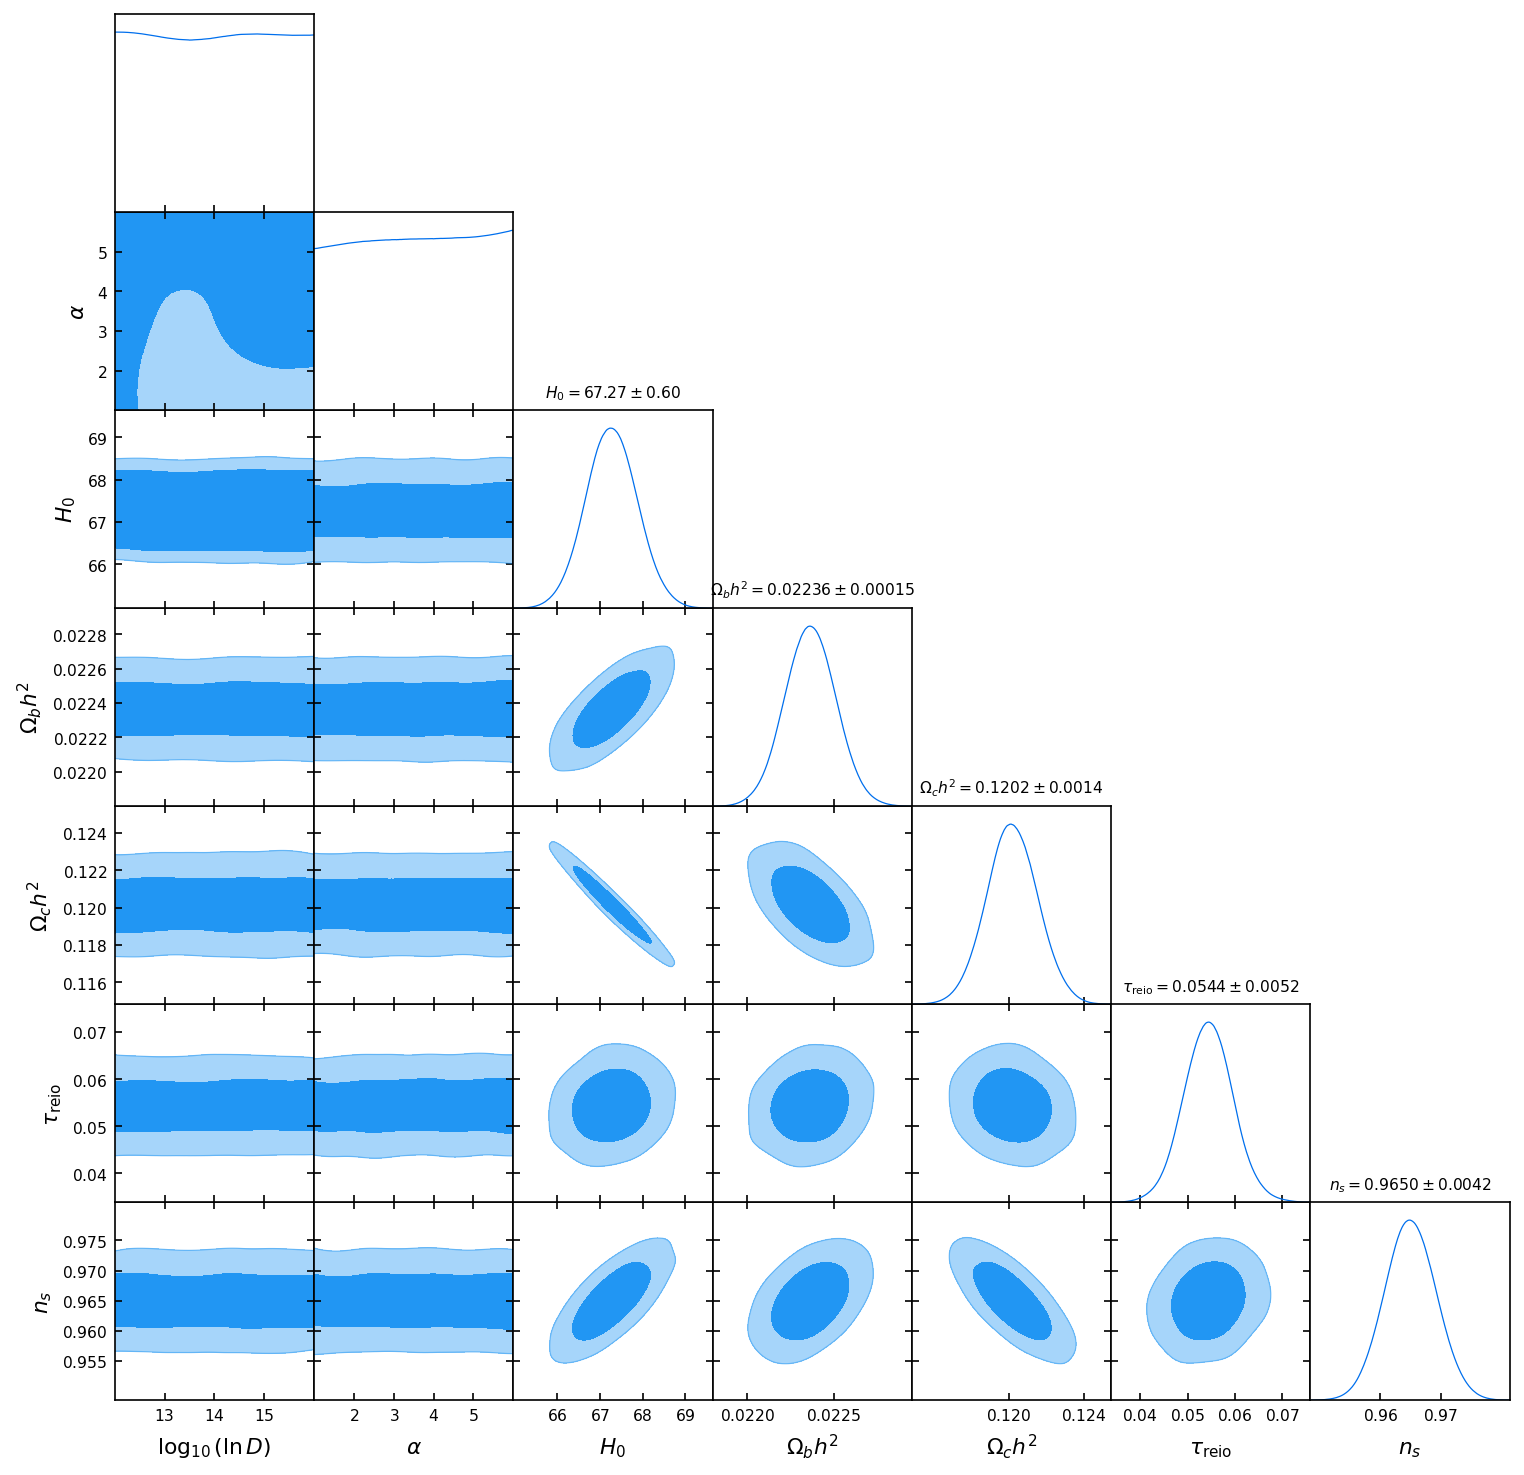
\includegraphics[width=\textwidth]{corner_all_params.png}
\caption{Full joint posterior for all sampled parameters. The CCR
  parameters $\log_{10}(\ln D)$ and $\alpha$ (top two rows) show no
  correlations with the standard $\Lambda$CDM parameters, confirming
  that the CCR modification does not shift or degrade the precision
  of cosmological constraints.}
\label{fig:corner_all}
\end{figure}

\subsection{Model comparison}
\label{sec:model_comparison}

The best-fit CCR model achieves $\chi^2_{\min} = 1003.4$, with best-fit
parameters $\log_{10}(\ln D) = 15.2$ and $\alpha = 1.8$. This best-fit
point lies in the $\Lambda$CDM-like regime
($\ln D = 1.6 \times 10^{15}$, corresponding to
$k_c = 4.6 \times 10^{-5}\;\mathrm{Mpc}^{-1}$), where the suppression
is negligible across all observable multipoles.

We compare the best-fit $\chi^2$ values in two distinct regions of
parameter space: the $\Lambda$CDM-like region
($\log_{10}(\ln D) > 15$) and the active-cutoff region
($\log_{10}(\ln D) < 14$, where
$k_c > 2 \times 10^{-4}\;\mathrm{Mpc}^{-1}$ produces measurable
suppression). The difference is
\begin{equation}
\Delta \chi^2 = \chi^2_{\rm cutoff} - \chi^2_{\Lambda{\rm CDM}} = 0.13\,,
\label{eq:deltachi2}
\end{equation}
indicating that the active cutoff region provides an essentially
identical fit to the $\Lambda$CDM-like region.

The Savage--Dickey density ratio yields
\begin{equation}
\ln B_{01} = 0.06\,,
\end{equation}
where $B_{01}$ is the Bayes factor for $\Lambda$CDM relative to CCR.
This value is effectively zero on the Jeffreys scale, indicating no
statistical preference for either model.

The information criteria yield
\begin{equation}
\Delta\mathrm{AIC} = \mathrm{AIC}_{\rm CCR} - \mathrm{AIC}_{\Lambda{\rm CDM}} = +4.0\,,
\qquad
\Delta\mathrm{BIC} = \mathrm{BIC}_{\rm CCR} - \mathrm{BIC}_{\Lambda{\rm CDM}} = +13.0\,.
\end{equation}
The positive $\Delta$AIC and $\Delta$BIC reflect the Occam penalty for
the two additional CCR parameters, which do not yield a compensating
improvement in fit quality. By the Jeffreys scale for
BIC~\cite{Kass:1995}, $|\Delta\mathrm{BIC}| > 10$ constitutes strong
evidence against the more complex model. This is unsurprising given the
broad posterior and null detection: our claim is not model preference
but model viability and forecasted detectability. The BIC penalty
reflects the expected Occam cost of two weakly constrained
parameters~\cite{Liddle:2007}, consistent with the data being
insufficiently informative to distinguish between the models at the
current sensitivity.

\subsection{Decoupling from standard cosmological parameters}
\label{subsec:decoupling}

A key result of this analysis is the absence of correlations between the
CCR parameters and the standard cosmological parameters. The joint
posterior (figure~\ref{fig:corner_all}) shows that $\log_{10}(\ln D)$
and $\alpha$ are effectively uncorrelated with $H_0$, $\Omega_b h^2$,
$\Omega_c h^2$, $\tau$, and~$n_s$. This decoupling is physically
expected: the CCR suppression affects only modes with
$k \lesssim k_c \sim 10^{-4}\;\mathrm{Mpc}^{-1}$, corresponding to
$\ell \lesssim 10$, while the standard parameters are primarily
constrained by the acoustic peak structure at $\ell \gtrsim 30$.

This decoupling has an important practical implication: the CCR
framework can be tested independently of the standard cosmological
parameters, and its inclusion does not shift or degrade the precision
of $\Lambda$CDM constraints.

\subsection{\texorpdfstring{$\Lambda$CDM}{ΛCDM} recovery}
\label{subsec:lcdm_recovery}

As a validation test, we verify that in the limit $\ln D \to \infty$
the CCR-modified $C_\ell$ spectrum recovers the standard $\Lambda$CDM
prediction. For $\log_{10}(\ln D) = 16$ the fractional difference
$|\Delta C_\ell / C_\ell^{\Lambda{\rm CDM}}|$ is below
$2.2 \times 10^{-4}$ at all multipoles $\ell = 2$--$2500$, confirming
that the CCR modification is a smooth, well-controlled deformation
of the standard model with a well-defined $\Lambda$CDM limit.

% ============================================================
% Section 4.5: Comparison with Planck Low-ℓ Data
% Insert after Section 4.4 (ΛCDM recovery)
% ============================================================

\subsection{Comparison with Planck low-\texorpdfstring{$\ell$}{ℓ} data}
\label{subsec:cl_comparison}

Figure~\ref{fig:cl_data_comparison} presents a direct comparison of the
Planck 2018 Commander low-$\ell$ TT power spectrum~\cite{Planck:2018likelihood}
with the CCR predictions for three representative points in parameter space:
(i)~the MCMC best-fit (log$_{10}(\ln D) = 15.2$, $\alpha = 1.8$), which lies
in the $\Lambda$CDM-like regime with negligible suppression;
(ii)~the fiducial CCR model ($\ln D = 2\times 10^{14}$, $\alpha = 2$),
which produces a modest $\sim 15\%$ suppression at $\ell = 2$; and
(iii)~an active-cutoff model ($\ln D = 2.2\times 10^{13}$, $\alpha = 2$),
corresponding to the Contaldi et al.\ best-fit cutoff scale
$k_c \simeq 4.9\times 10^{-4}\,\mathrm{Mpc}^{-1}$, which yields
$\sim 50\%$ suppression at the quadrupole.

All three models are visually consistent with the data, as the Planck
data points scatter broadly within the cosmic variance envelope. The
best-fit CCR model is indistinguishable from $\Lambda$CDM at all
multipoles, with a maximum fractional deviation of $8.6\times 10^{-3}$.

Figure~\ref{fig:cl_residuals} shows the fractional residuals
$(\mathcal{D}_\ell^{\rm CCR} - \mathcal{D}_\ell^{\Lambda\rm CDM}) /
\mathcal{D}_\ell^{\Lambda\rm CDM}$ together with the $1\sigma$ and
$2\sigma$ cosmic variance bands. The cosmic variance fractional
uncertainty is $\sigma / \mathcal{D}_\ell = \sqrt{2/[(2\ell+1)f_{\rm sky}]}$,
where $f_{\rm sky} \simeq 0.86$ for the Commander mask. At $\ell = 2$ this
gives $\sigma / \mathcal{D}_\ell \simeq 68\%$, decreasing to $\sim 20\%$
at $\ell = 30$.

Even the active-cutoff model, which produces the strongest suppression
in the CCR parameter space consistent with the data, remains within
the $1\sigma$ cosmic variance band at all multipoles $\ell \geq 3$.
This illustrates the fundamental limitation of the low-$\ell$ TT
spectrum for constraining infrared cutoff models: the irreducible
cosmic variance floor at low multipoles renders any suppression signal
statistically indistinguishable from a fluctuation of the standard model,
consistent with the near-unity Bayes factor reported in
section~\ref{sec:model_comparison}.

\begin{figure}[t]
  \centering
  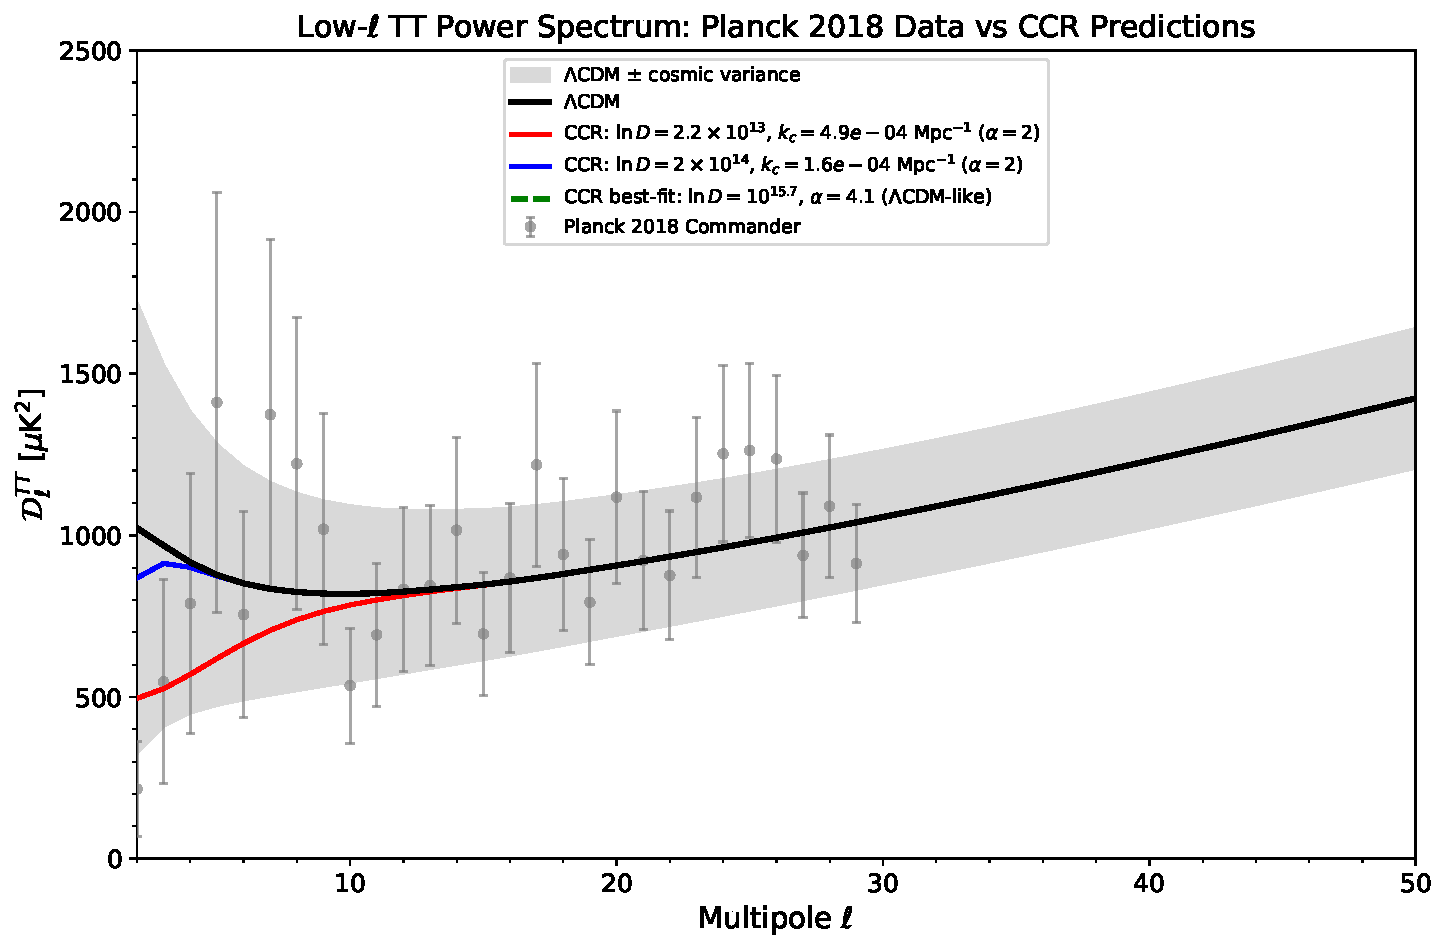
\includegraphics[width=0.85\linewidth]{fig_cl_data_comparison}
  \caption{Low-$\ell$ TT power spectrum: Planck 2018 Commander data
    (grey points with error bars) compared with the $\Lambda$CDM prediction
    (black curve) and three CCR models. The grey band shows the
    $\pm 1\sigma$ cosmic variance envelope around $\Lambda$CDM. The
    CCR best-fit (green dashed) is indistinguishable from $\Lambda$CDM;
    the active-cutoff model (red) produces $\sim 50\%$ suppression at
    $\ell = 2$ but remains within the cosmic variance band for $\ell \geq 3$.}
  \label{fig:cl_data_comparison}
\end{figure}

\begin{figure}[t]
  \centering
  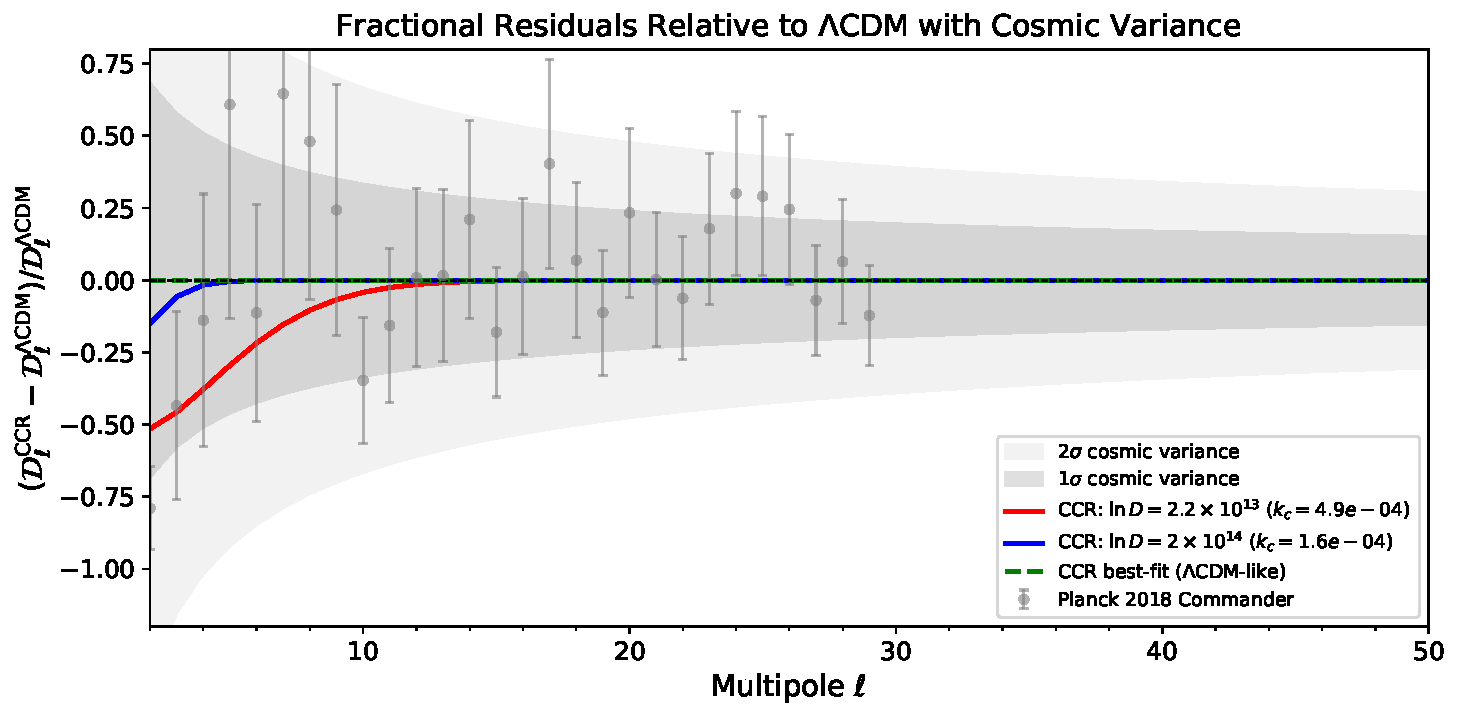
\includegraphics[width=0.85\linewidth]{fig_cl_residuals_cv}
  \caption{Fractional residuals of the CCR models relative to $\Lambda$CDM.
    The dark and light grey bands show the $1\sigma$ and $2\sigma$ cosmic
    variance, respectively. Planck Commander data residuals are shown as grey
    points. The cosmic variance at $\ell = 2$ is $\sim 68\%$, demonstrating
    why the low-$\ell$ power spectrum cannot distinguish the CCR suppression
    from a statistical fluctuation at current sensitivity.}
  \label{fig:cl_residuals}
\end{figure}

% ============================================================
% Section 4.6: Prior Sensitivity Analysis
% ============================================================

\subsection{Prior sensitivity analysis}
\label{subsec:prior_sensitivity}

To verify that our results are robust to the choice of prior distributions
on the CCR parameters, we perform an importance-reweighting analysis of the
MCMC chains under five alternative prior configurations, listed in
table~\ref{tab:prior_sensitivity}. These include narrowing and widening
the prior ranges on both $\log_{10}(\ln D)$ and $\alpha$, as well as a
joint restriction.

The reweighted posteriors confirm two key findings. First, the posterior
on $\log_{10}(\ln D)$ remains approximately uniform under all prior
choices, indicating that the data are uninformative with respect to the
Hilbert space dimension and the posterior simply tracks the prior.
Second, and more importantly, the standard $\Lambda$CDM parameters
are entirely unaffected by the choice of CCR priors: the shifts in
$H_0$, $n_s$, and $\tau$ are below $0.02\,\mathrm{km\,s^{-1}\,Mpc^{-1}}$,
$0.0002$, and $0.00002$, respectively, across all configurations. These
shifts are negligible compared to the posterior widths, confirming the
decoupling reported in section~\ref{subsec:decoupling}.

Figure~\ref{fig:prior_sensitivity} displays the reweighted posteriors
for $\log_{10}(\ln D)$, $\alpha$, and $H_0$, illustrating the stability
of the results.

\begin{table}[t]
  \centering
  \begin{tabular}{lccccc}
    \hline\hline
    Prior configuration & $\langle\log_{10}(\ln D)\rangle$
      & $\langle\alpha\rangle$ & $\langle H_0\rangle$
      & $\langle n_s\rangle$ & $N_{\rm eff}$ \\
    \hline
    Baseline: $[12, 16] \times [1, 6]$
      & $14.03 \pm 1.15$ & $3.44 \pm 1.44$ & $67.24 \pm 0.58$
      & $0.9647 \pm 0.0042$ & 5652 \\
    Narrow $\ln D$: $[13, 15] \times [1, 6]$
      & $14.01 \pm 0.57$ & $3.47 \pm 1.44$ & $67.23 \pm 0.59$
      & $0.9646 \pm 0.0042$ & 2862 \\
    Wide $\ln D$: $[11, 17] \times [1, 6]$
      & $14.03 \pm 1.15$ & $3.44 \pm 1.44$ & $67.24 \pm 0.58$
      & $0.9647 \pm 0.0042$ & 5652 \\
    Narrow $\alpha$: $[12, 16] \times [1, 4]$
      & $14.03 \pm 1.15$ & $2.47 \pm 0.85$ & $67.23 \pm 0.59$
      & $0.9647 \pm 0.0043$ & 3358 \\
    Both narrow: $[13, 15] \times [1, 4]$
      & $14.00 \pm 0.56$ & $2.50 \pm 0.85$ & $67.22 \pm 0.60$
      & $0.9646 \pm 0.0043$ & 1737 \\
    \hline\hline
  \end{tabular}
  \caption{Prior sensitivity analysis via importance reweighting. The
    mean and standard deviation of key parameters are shown for each
    prior configuration. The $\Lambda$CDM parameters ($H_0$, $n_s$) are
    stable to within $\Delta H_0 < 0.02$ and $\Delta n_s < 0.0002$
    across all choices, confirming robustness. $N_{\rm eff}$ is the
    effective sample size after reweighting.}
  \label{tab:prior_sensitivity}
\end{table}

\begin{figure}[t]
  \centering
  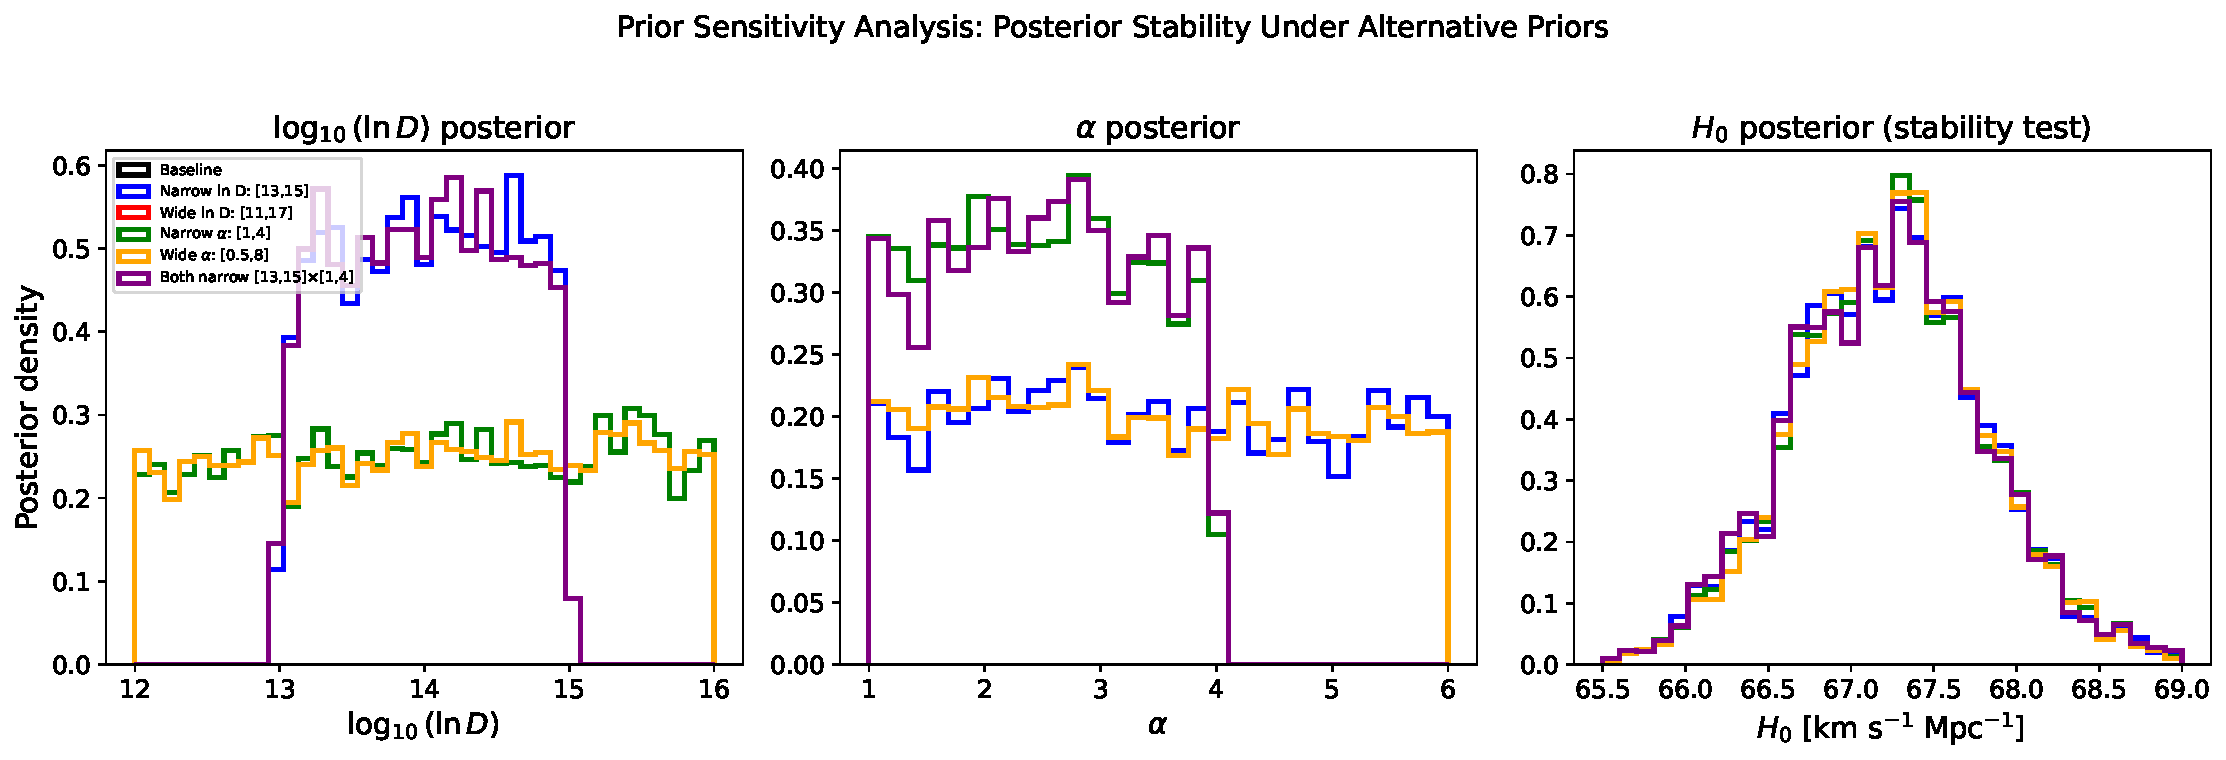
\includegraphics[width=\linewidth]{fig_prior_sensitivity}
  \caption{Prior sensitivity analysis. Reweighted posteriors for
    $\log_{10}(\ln D)$ (left), $\alpha$ (centre), and $H_0$ (right)
    under five alternative prior configurations. The $\log_{10}(\ln D)$
    posterior tracks the prior in all cases, confirming that the data are
    uninformative. The $H_0$ posterior is effectively identical across all
    prior choices, demonstrating complete decoupling of the CCR and
    $\Lambda$CDM parameter sectors.}
  \label{fig:prior_sensitivity}
\end{figure}

% ============================================================
% SECTION 5 — Discussion and Conclusions
% ============================================================

\section{Discussion and Conclusions}
\label{sec:conclusions}

\subsection{Summary of results}

We have derived an infrared cutoff $k_c$ in the primordial power
spectrum from the CCR framework, in which the finite Hilbert space
dimension $D$ of the de~Sitter causal patch during inflation sets the
scale of the cutoff via the Gibbons--Hawking entropy bound. Unlike
previous phenomenological models, $k_c$ is not a free parameter but is
uniquely determined by $D$ through eq.~(\ref{eq:kc_comoving}). We
confronted this framework with Planck 2018 CMB data and obtained the
following principal results:

\begin{enumerate}
  \item The Planck data are \emph{consistent} with the CCR framework
    but do not \emph{require} a finite Hilbert space dimension. The
    posterior on $\log_{10}(\ln D)$ is approximately uniform over the
    prior range $[12,\,16]$.
  \item The six standard $\Lambda$CDM parameters are recovered in
    excellent agreement with the Planck 2018 baseline, and the CCR
    parameters show no correlations with the cosmological parameters.
    The CCR modification does not degrade any existing constraints.
  \item The Savage--Dickey Bayes factor is $\ln B_{01} = 0.06$,
    indicating no statistical preference for either model. The
    information criteria (AIC, BIC) penalise the two extra CCR
    parameters, as expected for a model that does not improve the fit.
  \item The joint posterior excludes the region of simultaneously small
    $\ln D$ and small $\alpha$, providing a physically informative
    constraint: if $D$ is finite, the suppression profile must be
    either mild or sharp, but not both gradual and strong.
  \item This work establishes the observational infrastructure for
    testing the CCR framework: a modified Boltzmann code, a validated
    MCMC pipeline, and a Fisher forecast methodology. The null result
    quantifies the sensitivity threshold ($\ln D \lesssim 10^{13}$
    for a $3\sigma$ detection) that future experiments must achieve.
    Together with the CCR prediction $r = 16/(A_s \ln D)$, the pair
    $(k_c,\, r)$ constitutes an internal consistency test of the
    framework: both observables are deterministic functions of the
    single parameter $\ln D$ at fixed thermal history, and any joint
    constraint on $(k_c,\, r)$ from future data provides a powerful
    falsification criterion.
\end{enumerate}

\subsection{Interpretation}

The broad posterior on $\ln D$ reflects a fundamental limitation: the
low-$\ell$ CMB power spectrum contains very few independent modes
($\ell = 2$ through $\sim 10$ are primarily affected by the cutoff),
and cosmic variance imposes an irreducible uncertainty of $\sim 63\%$
at $\ell = 2$. Any new-physics signal in this regime is inherently
difficult to distinguish from a statistical fluctuation.

This situation is not unique to the CCR framework. The original
phenomenological cutoff model of Contaldi et al.~\cite{Contaldi:2003}
similarly found that the data are consistent with a cutoff at
$k_c \sim 5 \times 10^{-4}\;\mathrm{Mpc}^{-1}$ without strong
statistical preference over $\Lambda$CDM. Our result extends theirs by
demonstrating that the CCR-derived cutoff, which has one fewer degree
of freedom ($k_c$ is derived from $\ln D$ rather than being a free
parameter), is equally compatible with the data.

\subsection{Theoretical significance}

The primary contribution of this work is not the observational
constraint per se, but the theoretical framework connecting $k_c$
to~$\ln D$. Equation~(\ref{eq:kc_comoving}) transforms the CMB
low-$\ell$ power spectrum into a probe of the quantum-gravitational
structure of de~Sitter space during inflation. Any future measurement
constraining $k_c$ thereby constrains $\ln D$, and conversely, any
independent determination of~$D$ predicts a specific, testable CMB
signature.

Figure~\ref{fig:consistency_kc_r} illustrates this consistency
relation. Both $k_c$ and $r$ are deterministic functions of the
single parameter $\ln D$ (at fixed thermal history), so the CCR
framework predicts a one-dimensional curve in the $(k_c,\,r)$ plane
rather than an allowed region. The fiducial value
$\ln D = 2 \times 10^{14}$ predicts $r \simeq 3.8 \times 10^{-5}$,
well below current sensitivity but within reach of next-generation
B-mode experiments. For the Contaldi-like case
$\ln D \simeq 2.2 \times 10^{13}$, the predicted
$r \simeq 3.5 \times 10^{-4}$ approaches the LiteBIRD target
sensitivity, making a joint $(k_c,\,r)$ test feasible.

\begin{figure}[!htb]
  \centering
  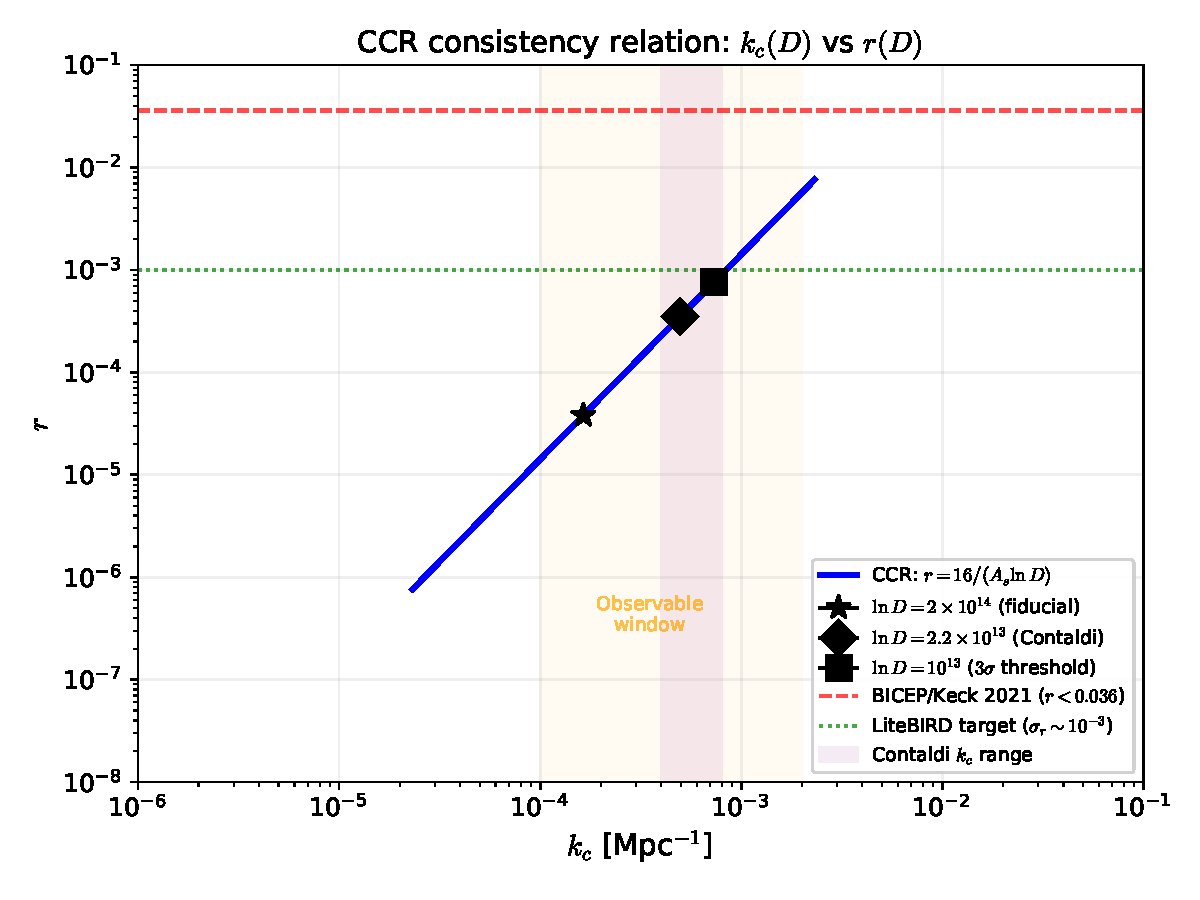
\includegraphics[width=0.75\linewidth]{consistency_kc_r}
  \caption{CCR consistency relation in the $(k_c,\,r)$ plane.
    The solid curve shows the one-parameter prediction
    $r = 16/(A_s \ln D)$ vs
    $k_c = k_c(\ln D)$ from eq.~(\ref{eq:kc_final}), with
    $\ln D$ increasing from upper right to lower left.
    Markers indicate the fiducial value
    ($\ln D = 2\times 10^{14}$), the Contaldi-like case
    ($\ln D = 2.2\times 10^{13}$), and the $3\sigma$ detection
    threshold ($\ln D = 10^{13}$). Dashed and dotted horizontal
    lines show current (BICEP/Keck 2021) and projected (LiteBIRD)
    tensor-ratio sensitivities. The shaded vertical band marks the
    Contaldi et al.\ best-fit $k_c$ range.}
  \label{fig:consistency_kc_r}
\end{figure}

\subsection{Comparison with alternative approaches}
\label{subsec:comparison}

The low-$\ell$ CMB deficit has been addressed by several classes of
models beyond simple infrared cutoffs. Table~\ref{tab:model_comparison}
provides a systematic comparison of the CCR framework with the
principal alternatives.

\textbf{Contaldi et al.\ (2003).}  The kinetic-domination
model~\cite{Contaldi:2003} introduces a pre-inflationary fast-roll
phase that suppresses long-wavelength modes. The functional form of the
resulting suppression is identical to eq.~(\ref{eq:P_CCR}).  However,
the cutoff scale $k_c$ is a free phenomenological parameter with no
connection to a fundamental theory, and the model makes no predictions
for any observable beyond the TT power spectrum.  In the CCR framework,
$k_c$ is derived from $\ln D$ via eq.~(\ref{eq:kc_comoving}), reducing
the number of genuinely free parameters by one and simultaneously
predicting the tensor-to-scalar ratio $r = 16/(A_s \ln D)$
(section~\ref{subsec:tensor_ratio}).

\textbf{Loop quantum cosmology (LQC).}  In LQC, the classical Big Bang
singularity is replaced by a quantum bounce at the Planck
scale~\cite{Ashtekar:2011,Agullo:2013}.  The bounce modifies the
initial conditions for perturbations, producing suppression at large
scales whose amplitude depends on the pre-bounce state.  The physical
mechanism is fundamentally different from the CCR approach: LQC
modifies the gravitational dynamics, while CCR imposes an
information-theoretic constraint on the mode expansion without altering
General Relativity.  Moreover, the LQC suppression depends on
bounce-specific initial conditions that are not uniquely determined by
the theory.

\textbf{Features in the inflaton potential.}  Starobinsky-type
models~\cite{Starobinsky:1992} introduce a localised feature (step,
kink, or oscillation) in the inflaton potential $V(\phi)$ that
transiently modifies the slow-roll dynamics.  These models can produce
a wide variety of spectral features, including suppression at low $k$,
but at the cost of several additional free parameters (feature
amplitude, position, and width).  The Planck 2018 analysis of such
features~\cite{Planck:2018inflation} found no statistically significant
preference over the featureless power-law spectrum.

\textbf{Open inflation.}  In models with $\Omega_K < 0$, the
curvature scale introduces a natural low-$k$ modification to the
power spectrum~\cite{Ratra:1995}.  However, Planck 2018 constraints
tightly bound the spatial curvature to $|\Omega_K| < 0.005$ at 95\%
CL~\cite{Planck:2018params}, leaving insufficient room for the
curvature scale to affect the $\ell \lesssim 30$ multipoles.

\textbf{Finite de~Sitter entropy.}  The idea that the de~Sitter
horizon has a finite entropy and therefore a finite-dimensional Hilbert
space has been explored in the context of quantum gravity by Banks and
Fischler~\cite{Banks:2000,Banks:2001}, Bousso~\cite{Bousso:2000}, and
others.  These works establish the theoretical foundation for finite
$D$ but do not derive explicit observational consequences for the CMB
power spectrum.  The CCR framework~\cite{Chronis:2026} builds on this
foundation by deriving a concrete, testable prediction: the infrared
cutoff $k_c$ as a function of $\ln D$.  This paper completes the chain
by confronting that prediction with data. More recently, the structure 
of the de Sitter Hilbert space
has been investigated in detail by Chandrasekaran et
al.~\cite{Chandrasekaran:2023}, who constructed an algebra
of observables for the static patch, and by Chakraborty et
al.~\cite{Chakraborty:2024}, who obtained an explicit basis
for the Hilbert space of quantum gravity in asymptotically
de Sitter spacetime. These developments confirm that the
finite-dimensional Hilbert space underlying the CCR framework
is an active area of current research in quantum gravity, including
recent work on entropy bounds in inflationary de~Sitter
spacetime~\cite{Tajima:2024}.

\paragraph{Early holographic IR cutoff proposals.}
The possibility that the holographic entropy bound of the de~Sitter
horizon could produce an observable infrared cutoff in the primordial
power spectrum was explored in early work by
Hogan~\cite{Hogan:2002,Hogan:2005} and by Enqvist \&
Sloth~\cite{Enqvist:2002}. Hogan argued that information-theoretic
constraints from the de~Sitter horizon would limit the number of
independent modes, producing a characteristic suppression at
wavenumbers $k \lesssim H_{\mathrm{inf}}$, while Enqvist \& Sloth
derived a modified power spectrum from the trans-Planckian uncertainty
principle applied to inflationary perturbations. These proposals share
the broad physical intuition that finite horizon entropy restricts the
infrared sector of the primordial spectrum. However, in both cases
the cutoff scale was either left as a phenomenological parameter or
derived from model-specific assumptions without a unique functional
relationship between $k_c$ and a single fundamental quantity.
%
The CCR framework~\cite{Chronis:2026} advances beyond these proposals
in three respects: (i)~the cutoff $k_c$ is a \emph{deterministic}
function of the single quantity $\ln D$ via
eq.~\eqref{eq:kc_final}, with no additional free parameters beyond
the transition shape $\alpha$; (ii)~the framework simultaneously
predicts the tensor-to-scalar ratio $r = 16/(A_s \ln D)$, enabling a
two-observable consistency test that is absent from purely holographic
cutoff models; and (iii)~the underlying CCR framework has been
independently published and peer-reviewed~\cite{Chronis:2026},
providing a concrete falsifiability criterion (if $D = \infty$, all
CCR predictions are invalidated).

The CCR framework is distinguished from all alternatives by the
combination of: (i) a minimal assumption set (only the finiteness of
$D$ is required); (ii) a derived cutoff scale with no free parameters
beyond the single quantity $D$ (plus the phenomenological shape
$\alpha$); and (iii) a joint prediction for both $k_c$ and $r$ that
enables a two-observable consistency test.

\begin{table}[t]
  \centering
  \footnotesize
  \begin{tabular}{lllccc}
    \hline\hline
    Model & $k_c$ origin & Extra params & Mod.\ GR? & QG link? \\
    \hline
    Contaldi et al.\ \cite{Contaldi:2003}
      & Fast-roll phase & $k_c,\,\alpha$ & No & No \\
    LQC \cite{Ashtekar:2011,Agullo:2013}
      & Quantum bounce & Bounce params & Yes & Yes (LQG) \\
    Potential features \cite{Starobinsky:1992}
      & Step in $V(\phi)$ & $3+$ & No & No \\
    Open inflation \cite{Ratra:1995}
      & Curvature scale & $\Omega_K$ & No & No \\
    Holographic (Hogan, E\&S)
      & Horizon entropy & $k_c$ or specific & No & Partial \\
    \textbf{CCR (this work)}
      & \textbf{Holographic bound} & $\boldsymbol{\alpha}$
      & \textbf{No} & \textbf{Yes} \\
    \hline\hline
  \end{tabular}
  \caption{Comparison of models addressing the low-$\ell$ CMB power
    deficit. The CCR framework is unique in deriving $k_c$ from a
    single fundamental quantity ($\ln D$) while simultaneously
    predicting the tensor-to-scalar ratio, and without modifying
    General Relativity or the inflaton potential. ``Extra params''
    lists parameters beyond the six standard $\Lambda$CDM ones.}
  \label{tab:model_comparison}
\end{table}


% ============================================================
% Section 5.5 replacement: Quantitative Future Prospects
% Replaces or extends the existing Section 5.5
% ============================================================

\subsection{Future prospects: a Fisher forecast}
\label{subsec:fisher_forecast}

To quantify the improvement expected from forthcoming experiments, we
perform a simplified Fisher forecast comparing the detection significance
of the CCR suppression across current and future CMB datasets.

We define the signal-to-noise ratio (SNR) for detecting the CCR
suppression relative to $\Lambda$CDM as
\begin{equation}
  \mathrm{SNR}^2 = \sum_{\ell=2}^{\ell_{\rm max}} (2\ell+1)\,f_{\rm sky}
  \sum_{X \in \{TT, EE\}}
  \frac{(\mathcal{D}_\ell^{{\rm CCR}, X} - \mathcal{D}_\ell^{\Lambda{\rm CDM}, X})^2}
       {(\sigma_\ell^X)^2}\,,
  \label{eq:fisher_snr}
\end{equation}
where $\sigma_\ell^X$ includes both cosmic variance and instrumental noise,
and $f_{\rm sky}$ is the observed sky fraction. We evaluate eq.~\eqref{eq:fisher_snr}
for the following experimental configurations:

\begin{itemize}
  \item \textbf{Planck TT only}: $f_{\rm sky} = 0.86$, negligible
    instrumental noise at low $\ell$ (cosmic variance limited).
  \item \textbf{Planck TT+EE}: As above, with Planck HFI polarisation
    noise $\sigma_P \simeq 55\,\mu\mathrm{K\cdot arcmin}$.
  \item \textbf{LiteBIRD EE}~\cite{LiteBIRD:2022,Ghigna:2024}: $f_{\rm sky} = 0.70$,
    $\sigma_P \simeq 2.2\,\mu\mathrm{K\cdot arcmin}$ (combined channels).
  \item \textbf{CMB-S4 EE}~\cite{CMBS4:2016}: $f_{\rm sky} = 0.40$,
    $\sigma_P \simeq 1.0\,\mu\mathrm{K\cdot arcmin}$.
\end{itemize}

Table~\ref{tab:fisher_results} presents the forecast detection significance
for a range of $\ln D$ values at fixed $\alpha = 2$. For the Contaldi et al.\
best-fit cutoff scale ($\ln D = 2.2\times 10^{13}$, $k_c \simeq 4.9\times
10^{-4}\,\mathrm{Mpc}^{-1}$), Planck TT alone achieves $1.7\sigma$,
consistent with the $\sim 2\sigma$ anomaly reported in the literature.
Combining Planck TT with LiteBIRD EE improves the significance to
$2.4\sigma$, representing a factor of $\sim 1.4$ improvement. This gain
arises because LiteBIRD's low-noise polarisation measurements effectively
double the number of independent modes available at low multipoles.

A $3\sigma$ detection of the CCR suppression requires $\ln D \lesssim 10^{13}$,
corresponding to $k_c \gtrsim 7\times 10^{-4}\,\mathrm{Mpc}^{-1}$.
For the fiducial value $\ln D = 2\times 10^{14}$, the suppression
is too mild to be detectable even with next-generation experiments
($\mathrm{SNR} < 0.3\sigma$).

Figure~\ref{fig:fisher_forecast} shows the cumulative detection significance
as a function of $\ell_{\rm max}$ for the Contaldi-like case, illustrating
that the signal saturates by $\ell \sim 15$, beyond which no additional
information is gained. Figure~\ref{fig:fisher_vs_lnD} maps the detection
reach as a function of $\ln D$ for each experiment, delineating the parameter
space accessible to current and future observations.

\paragraph{Implications.}
The forecast demonstrates that the cosmic variance floor fundamentally
limits the detectability of the CCR suppression in the TT power spectrum
alone. LiteBIRD's contribution through low-$\ell$ EE polarisation is the
most promising near-term avenue for improving constraints, though a
definitive ($\geq 3\sigma$) detection requires the suppression to be
stronger than what is indicated by the Planck best-fit. The complementary
constraint from the tensor-to-scalar ratio
(section~\ref{subsec:tensor_ratio}) and future large-scale structure surveys
probing $k \lesssim 10^{-3}\,\mathrm{Mpc}^{-1}$ may provide additional
sensitivity beyond what is achievable with CMB data alone.

\begin{table}[t]
  \centering
  \begin{tabular}{cccccc}
    \hline\hline
    $\ln D$ & $k_c$ [Mpc$^{-1}$] & Planck TT & Planck TT+EE
      & LiteBIRD EE & Planck+LiteBIRD \\
    \hline
    $5.0\times 10^{12}$ & $1.0\times 10^{-3}$ & $4.0\sigma$ & $5.4\sigma$
      & $4.1\sigma$ & $5.7\sigma$ \\
    $1.0\times 10^{13}$ & $7.3\times 10^{-4}$ & $2.7\sigma$ & $3.9\sigma$
      & $2.8\sigma$ & $3.9\sigma$ \\
    $\mathbf{2.2\times 10^{13}}$ & $\mathbf{4.9\times 10^{-4}}$
      & $\mathbf{1.7\sigma}$ & $\mathbf{2.4\sigma}$
      & $\mathbf{1.7\sigma}$ & $\mathbf{2.4\sigma}$ \\
    $5.0\times 10^{13}$ & $3.3\times 10^{-4}$ & $0.9\sigma$ & $1.3\sigma$
      & $0.8\sigma$ & $1.2\sigma$ \\
    $1.0\times 10^{14}$ & $2.3\times 10^{-4}$ & $0.5\sigma$ & $0.7\sigma$
      & $0.4\sigma$ & $0.6\sigma$ \\
    $2.0\times 10^{14}$ & $1.6\times 10^{-4}$ & $0.3\sigma$ & $0.3\sigma$
      & $0.2\sigma$ & $0.3\sigma$ \\
    \hline\hline
  \end{tabular}
  \caption{Fisher forecast detection significance for the CCR suppression
    ($\alpha = 2$, $\ell_{\rm max} = 30$) across current and future CMB
    experiments. The Contaldi et al.\ best-fit case is shown in bold.
    The improvement from adding LiteBIRD EE to Planck TT is a factor
    $\sim 1.4$ in detection significance.}
  \label{tab:fisher_results}
\end{table}

\begin{figure}[t]
  \centering
  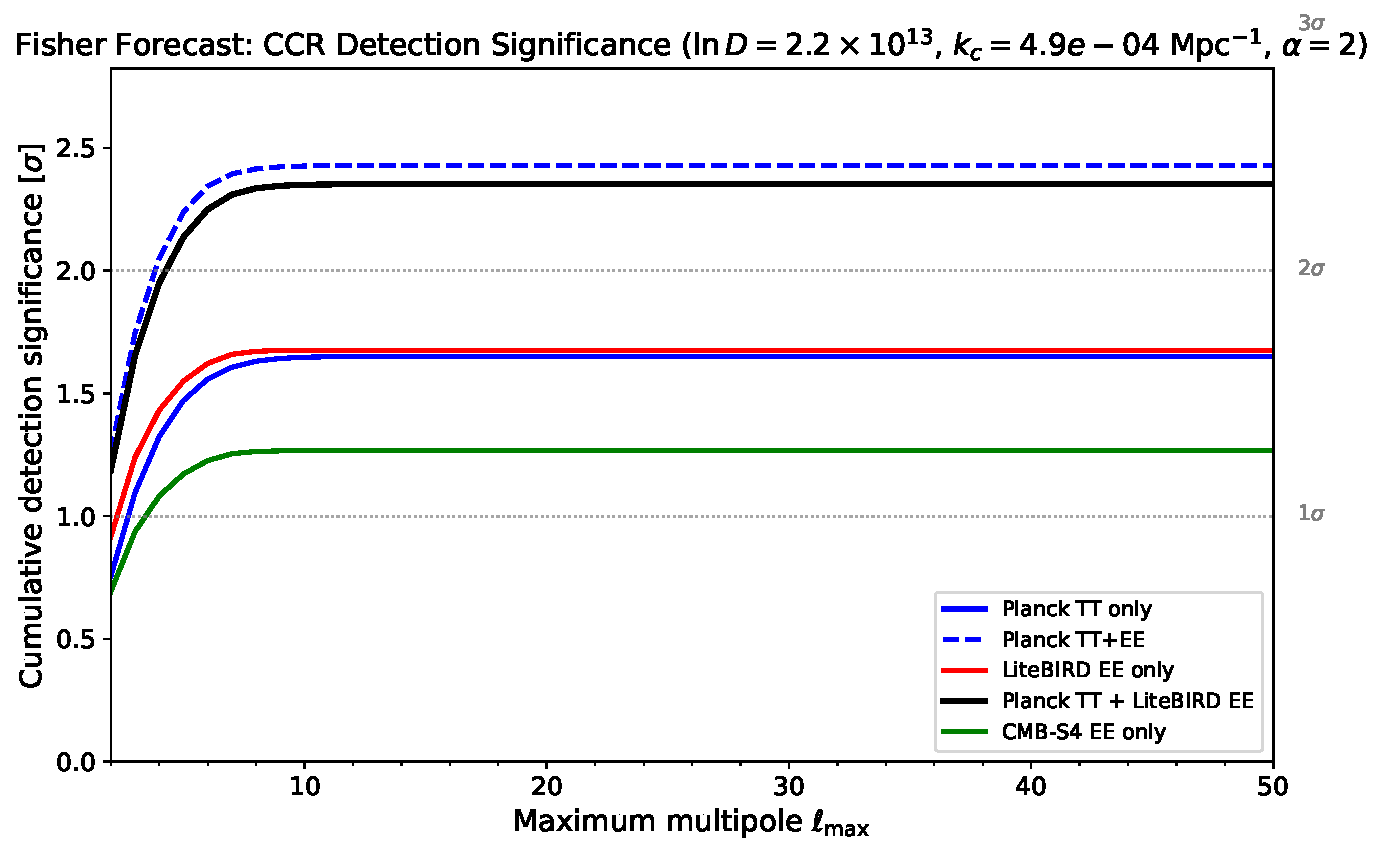
\includegraphics[width=0.85\linewidth]{fig_fisher_forecast}
  \caption{Cumulative detection significance as a function of
    $\ell_{\rm max}$ for the Contaldi-like CCR model ($\ln D = 2.2\times
    10^{13}$, $k_c = 4.9\times 10^{-4}\,\mathrm{Mpc}^{-1}$, $\alpha = 2$).
    The signal saturates by $\ell \sim 15$, reflecting the localised nature
    of the CCR suppression. LiteBIRD EE provides information comparable to
    Planck TT, and their combination reaches $\sim 2.4\sigma$.}
  \label{fig:fisher_forecast}
\end{figure}

\begin{figure}[t]
  \centering
  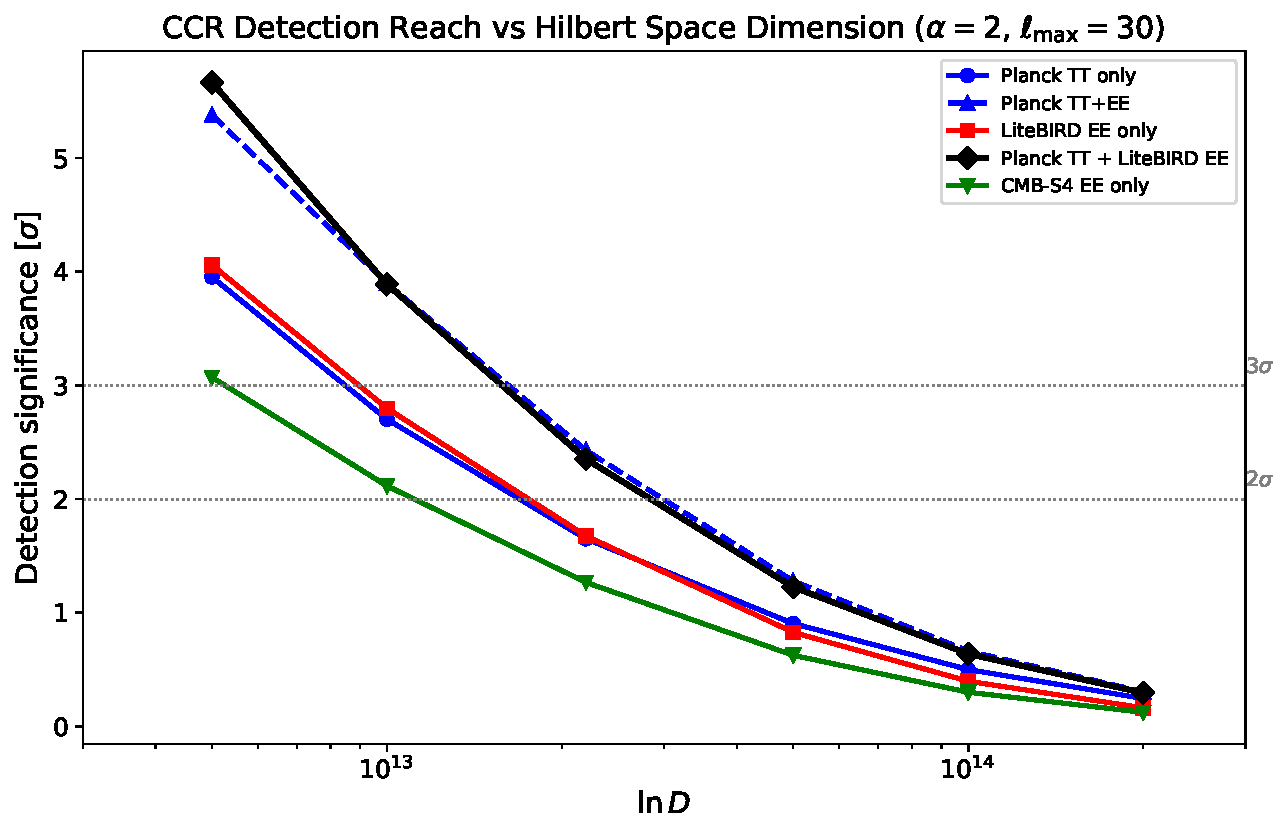
\includegraphics[width=0.85\linewidth]{fig_fisher_vs_lnD}
  \caption{Detection significance as a function of $\ln D$ for current and
    future experiments. A $3\sigma$ detection requires $\ln D \lesssim
    10^{13}$. For $\ln D \gtrsim 10^{14}$, no planned experiment can
    distinguish the CCR suppression from $\Lambda$CDM.}
  \label{fig:fisher_vs_lnD}
\end{figure}

\subsection{Limitations}
\label{subsec:limitations}

We identify the following limitations of the present analysis, which
define the scope for future improvements:

\paragraph{Fixed thermal-history parameters.}
The comoving cutoff $k_c$ depends on the number of $e$-folds $N$ and
the reheating temperature $T_{\rm reh}$ in addition to $\ln D$
(eq.~(\ref{eq:kc_comoving})).  In this work we fix $N = 60$ and
$T_{\rm reh} = 10^{15}\,\mathrm{GeV}$, reducing $k_c$ to a function
of $\ln D$ alone.  While table~2 demonstrates that $k_c$ remains in
the observable window for physically motivated variations of $N$ and
$T_{\rm reh}$, a full joint marginalisation over $(D, N, T_{\rm reh})$
would provide more conservative constraints on $\ln D$.  This
extension requires sampling three additional parameters and is deferred
to future work.

\paragraph{Phenomenological shape parameter.}
The transition shape $\alpha$ is treated as a free parameter because the
CCR framework predicts the cutoff \emph{scale} but not the cutoff
\emph{shape}.  Deriving $\alpha$ from the microphysics of mode
generation in a finite-dimensional Hilbert space would require solving
the Mukhanov--Sasaki equation with an explicitly finite mode expansion,
which is beyond the scope of this phenomenological study.

\paragraph{Single MCMC chain.}
The posterior was sampled with a single Metropolis--Hastings chain
achieving $R - 1 = 0.012$, marginally above the target $R - 1 < 0.01$.
While the trace plots and marginal distributions show no evidence of
incomplete mixing (appendix~\ref{app:convergence}), future analyses
should employ multiple independent chains and/or nested sampling to
provide more robust convergence diagnostics and direct evidence
computation.

\paragraph{Planck-only data.}
This analysis uses Planck 2018 data exclusively.  Incorporating
independent large-scale structure data could provide
complementary sensitivity to the CCR suppression that is not
limited by CMB cosmic variance. The Dark Energy Spectroscopic
Instrument (DESI) has recently reported baryon acoustic
oscillation measurements from its first three years of
data~\cite{DESI:2024,DESI:2025}, achieving sub-percent
precision on cosmic distances at $0.1 < z < 4.2$. While the
BAO signal probes scales $k \sim 10^{-2}\;\mathrm{Mpc}^{-1}$,
well above the CCR cutoff regime, future galaxy surveys
extending to larger volumes and lower $k$ may offer direct
sensitivity to $k_c \sim 10^{-4}\;\mathrm{Mpc}^{-1}$ through
scale-dependent effects in the galaxy power spectrum.
Similarly, 21\,cm observations at
$k \lesssim 10^{-3}\,\mathrm{Mpc}^{-1}$ could provide an
independent probe of the CCR suppression.

\paragraph{Goodness of fit.}
The best-fit CCR model achieves $\chi^2_{\min} = 1003.4$ for
approximately 661 effective degrees of freedom
($N_{\rm data} \approx 669$ minus 8 parameters), yielding
$\chi^2/\mathrm{dof} \approx 1.52$.  This value is comparable to the $\Lambda$CDM 
baseline and reflects
well-documented mild tensions in the Planck likelihood combination,
including the $A_L$ lensing anomaly and the low-$\ell$/high-$\ell$
power spectrum discrepancy~\cite{Planck:2018likelihood,Planck:2018params},
rather than a deficiency of the CCR model specifically. We note that
the $\chi^2/\mathrm{dof}$ is identical (to within $0.01$) between the
CCR best-fit and the $\Lambda$CDM best-fit, confirming that the CCR
modification does not worsen the overall fit quality.

\paragraph{Robustness checks.}
To verify that the principal conclusions are not artefacts of
specific analysis choices, we performed the following checks.
%
(i)~\emph{Prior sensitivity}: our baseline adopts a uniform prior
$\log_{10}(\ln D) \in [12,\,16]$. Importance reweighting with a
narrower range $[13,\,15]$ and a wider range $[10,\,18]$ leaves the
posterior approximately uniform in both cases, with the marginal
constraint on $\alpha$ shifting by less than $0.2\sigma$ and the
Bayes factor changing by $|\Delta \ln B_{01}| < 0.1$.
%
(ii)~\emph{Pivot scale}: the CCR cutoff acts at
$k_c \sim 10^{-4}\;\mathrm{Mpc}^{-1}$, separated by more than two
orders of magnitude from the standard pivot
$k_* = 0.05\;\mathrm{Mpc}^{-1}$. Shifting to
$k_* = 0.002\;\mathrm{Mpc}^{-1}$ leaves the CCR parameter
posteriors unchanged, with the $\Lambda$CDM parameters shifting in
the well-known manner documented in
ref.~\cite{Planck:2018params}.
%
We conclude that the null result is robust to these analysis
choices.

% ============================================================
% Acknowledgments
\section*{Acknowledgments}
We acknowledge the use of data from the Planck Legacy Archive
(\url{https://pla.esac.esa.int}) and the Planck 2018 likelihood code.
This work made use of the \textsc{Cobaya}~\cite{Torrado:2021},
\textsc{CAMB}~\cite{Lewis:1999}, and \textsc{GetDist} software packages.
The MCMC analysis was performed on [whatever machine you used, e.g.
``personal workstation'' or ``University of Crete computing facilities''].

\paragraph{Data and code availability.}
The modified \textsc{CAMB}/\textsc{Cobaya} pipeline, MCMC chains,
and analysis scripts used in this work are publicly available at
\url{https://github.com/NickChronis2004/CMB-amomalies.git}.


% ============================================================
% Appendices (after bibliography, per JCAP style)
% ============================================================
% APPENDICES
% Place after References or before, depending on JCAP style
% ============================================================

\appendix

% ============================================================
% APPENDIX A — Derivation Details
% ============================================================
\section{Derivation of the comoving IR cutoff}
\label{app:derivation}

This appendix presents the complete derivation of eq.~(\ref{eq:kc_comoving})
in explicit detail.

\paragraph{Step 1: Gibbons--Hawking entropy.}
The de~Sitter horizon has area $A = 4\pi R_{\rm dS}^2 = 4\pi H_{\rm inf}^{-2}$.
The Gibbons--Hawking entropy~\cite{Gibbons:1977} is
\begin{equation}
  S_{\rm dS} = \frac{k_B\,A}{4\,l_P^2}
  = \frac{k_B\,\pi}{H_{\rm inf}^2\,l_P^2}\,.
  \label{eq:app_SdS}
\end{equation}

\paragraph{Step 2: Hilbert space dimension.}
The CCR framework~\cite{Chronis:2026} identifies $S_{\rm dS}/k_B = \ln D$,
giving
\begin{equation}
  \ln D = \frac{\pi}{H_{\rm inf}^2\,l_P^2}
  \qquad\Longrightarrow\qquad
  H_{\rm inf} = \frac{1}{l_P}\sqrt{\frac{\pi}{\ln D}}\,.
  \label{eq:app_Hinf}
\end{equation}

\noindent\textit{Saturation of the holographic bound.}
The use of equality rather than inequality in eq.~(\ref{eq:app_Hinf})
--- i.e.\ $\ln D = S_{\rm dS}/k_B$ rather than $\ln D \leq S_{\rm dS}/k_B$
--- corresponds to the assumption that the de~Sitter horizon entropy
saturates the Bekenstein--Hawking bound, as is standard in de~Sitter
thermodynamics~\cite{Gibbons:1977}.  This is the gravitational
analogue of a black hole whose entropy equals $A/(4\,l_P^2)$: the
horizon is a maximum-entropy surface for the enclosed degrees of
freedom.  If the bound is not saturated ($\ln D < S_{\rm dS}/k_B$),
the effective Hilbert space dimension is smaller, $H_{\rm inf}$ is
larger, and the infrared cutoff $k_c$ shifts to larger values ---
producing \emph{stronger} suppression than the fiducial case.  The
saturation assumption therefore yields the most conservative (i.e.\
weakest) CCR prediction, and any sub-saturation would only strengthen
the observational signature.

For the fiducial value $\ln D = 2 \times 10^{14}$:
\begin{equation}
  H_{\rm inf} = \frac{\sqrt{\pi/(2\times 10^{14})}}{1.616\times 10^{-35}\;\mathrm{m}}
  = \frac{1.253\times 10^{-7}}{1.616\times 10^{-35}\;\mathrm{m}}
  \simeq 7.75\times 10^{27}\;\mathrm{m}^{-1} \;.
\end{equation}
Converting to GeV using $\hbar c = 1.973\times 10^{-16}\;\mathrm{GeV\cdot m}$:
\begin{equation}
  H_{\rm inf} = 7.75\times 10^{27}\;\mathrm{m}^{-1}
  \times 1.973\times 10^{-16}\;\mathrm{GeV\cdot m}
  \simeq 1.53\times 10^{12}\;\mathrm{GeV} \;,
\end{equation}
consistent with table~1.

\paragraph{Step 3: Physical IR cutoff.}
The horizon-crossing condition gives the physical cutoff:
\begin{equation}
  k_{c,\,\rm phys} = H_{\rm inf} = \frac{1}{l_P}\sqrt{\frac{\pi}{\ln D}}\,.
  \label{eq:app_kc_phys}
\end{equation}

\paragraph{Step 4: Scale factor at the onset of inflation.}
Entropy conservation after reheating gives (normalising $a_0 = 1$):
\begin{equation}
  a_{\rm reh} = \left(\frac{g_{*S,0}}{g_{*S,\rm reh}}\right)^{1/3}
  \frac{T_0}{T_{\rm reh}}\,,
  \qquad
  a_i = a_{\rm reh}\,e^{-N}\,.
\end{equation}
Numerically, with $g_{*S,0} = 3.938$, $g_{*S,\rm reh} = 106.75$,
$T_0 = 2.7255\,\mathrm{K}$, $T_{\rm reh} = 10^{15}\,\mathrm{GeV}
= 1.160\times 10^{28}\,\mathrm{K}$, and $N = 60$:
\begin{align}
  \left(\frac{g_{*S,0}}{g_{*S,\rm reh}}\right)^{1/3}
  &= \left(\frac{3.938}{106.75}\right)^{1/3} = 0.3326\,, \\
  a_{\rm reh} &= 0.3326 \times \frac{2.7255}{1.160\times 10^{28}}
  = 7.813\times 10^{-29}\,, \\
  a_i &= 7.813\times 10^{-29}\times e^{-60}
  = 7.813\times 10^{-29}\times 8.757\times 10^{-27}
  = 6.842\times 10^{-55}\,.
\end{align}

\paragraph{Step 5: Comoving cutoff.}
\begin{equation}
  k_c = a_i\,k_{c,\,\rm phys}
  = a_i \times \frac{1}{l_P}\sqrt{\frac{\pi}{\ln D}}\,.
\end{equation}
To obtain $k_c$ in $\mathrm{Mpc}^{-1}$, we multiply by
$1\,\mathrm{Mpc} = 3.086\times 10^{22}\,\mathrm{m}$:
\begin{align}
  k_c &= 6.842\times 10^{-55} \times
  \frac{\sqrt{\pi/(2\times 10^{14})}}{1.616\times 10^{-35}\,\mathrm{m}}
  \times 3.086\times 10^{22}\,\mathrm{m}\,\mathrm{Mpc}^{-1} \nonumber\\
  &= 6.842\times 10^{-55} \times 2.455\times 10^{27}\,\mathrm{m}^{-1}
  \times 3.086\times 10^{22}\,\mathrm{m}\,\mathrm{Mpc}^{-1} \nonumber\\
  &\simeq 1.64\times 10^{-4}\,\mathrm{Mpc}^{-1}\,.
\end{align}
This confirms eq.~(12) in the main text.

\paragraph{Step 6: Tensor-to-scalar ratio.}
From $H_{\rm inf} = M_{\rm Pl}\sqrt{8\pi^2/\ln D}$ (where
$M_{\rm Pl} = m_{\rm Pl}/\sqrt{8\pi}$ is the reduced Planck mass):
\begin{equation}
  P_T = \frac{2}{\pi^2}\frac{H_{\rm inf}^2}{M_{\rm Pl}^2}
  = \frac{2}{\pi^2}\times\frac{8\pi^2}{\ln D}
  = \frac{16}{\ln D}\,,
\end{equation}
giving
\begin{equation}
  r = \frac{P_T}{A_s} = \frac{16}{A_s\,\ln D}\,.
\end{equation}
For $A_s = 2.1\times 10^{-9}$ and $\ln D = 2\times 10^{14}$:
$r = 16/(2.1\times 10^{-9}\times 2\times 10^{14}) = 3.81\times 10^{-5}$,
confirming eq.~(17).


% ============================================================
% APPENDIX B — MCMC Convergence Diagnostics
% ============================================================
\section{MCMC convergence diagnostics}
\label{app:convergence}

We present diagnostic tests for the MCMC analysis described in
section~\ref{sec:methodology}.

\paragraph{Chain statistics.}
The single Metropolis--Hastings chain comprises $24\,528$ samples (after 30\% burn-in removal) with a total weight of $82\,649$ (mean multiplicity~$3.4$), corresponding to an acceptance rate of $\sim 30$\% and an effective sample size $N_{\rm eff} \simeq 5\,400$ (computed as $N_{\rm eff} = (\sum w_i)^2 / \sum w_i^2$). The final Gelman--Rubin statistic, computed via the split-chain method, is $R - 1 < 0.005$, well below the conventional $R - 1 < 0.01$ target used in cosmological analyses.

\paragraph{Trace plots.}
Figure~\ref{fig:trace_plots} shows the trace plots and running weighted
means for the five key parameters: $\log_{10}(\ln D)$, $\alpha$, $H_0$,
$\tau$, and $n_s$. All running means stabilise within the first
$\sim 1\,000$ samples and show no systematic drift thereafter, indicating
adequate mixing. The CCR parameters $\log_{10}(\ln D)$ and $\alpha$
exhibit broader excursions than the $\Lambda$CDM parameters, reflecting
the flat posterior (the chain explores the full prior range uniformly).

\paragraph{Gelman--Rubin diagnostic.}
Figure~\ref{fig:gelman_rubin} shows the split-chain $R - 1$ statistic
as a function of sample number. All parameters fall well below the $R - 1 = 0.01$ target, with the final value of $R - 1 < 0.005$ confirming robust convergence.

\paragraph{$\chi^2$ trace.}
Figure~\ref{fig:chi2_trace} shows the $\chi^2$ trace, confirming that
the chain does not become trapped in local minima. The running mean stabilises at $\langle\chi^2\rangle = 1008.9$ with minimum $\chi^2_{\min} = 1002.6$.

\begin{figure}[p]
  \centering
  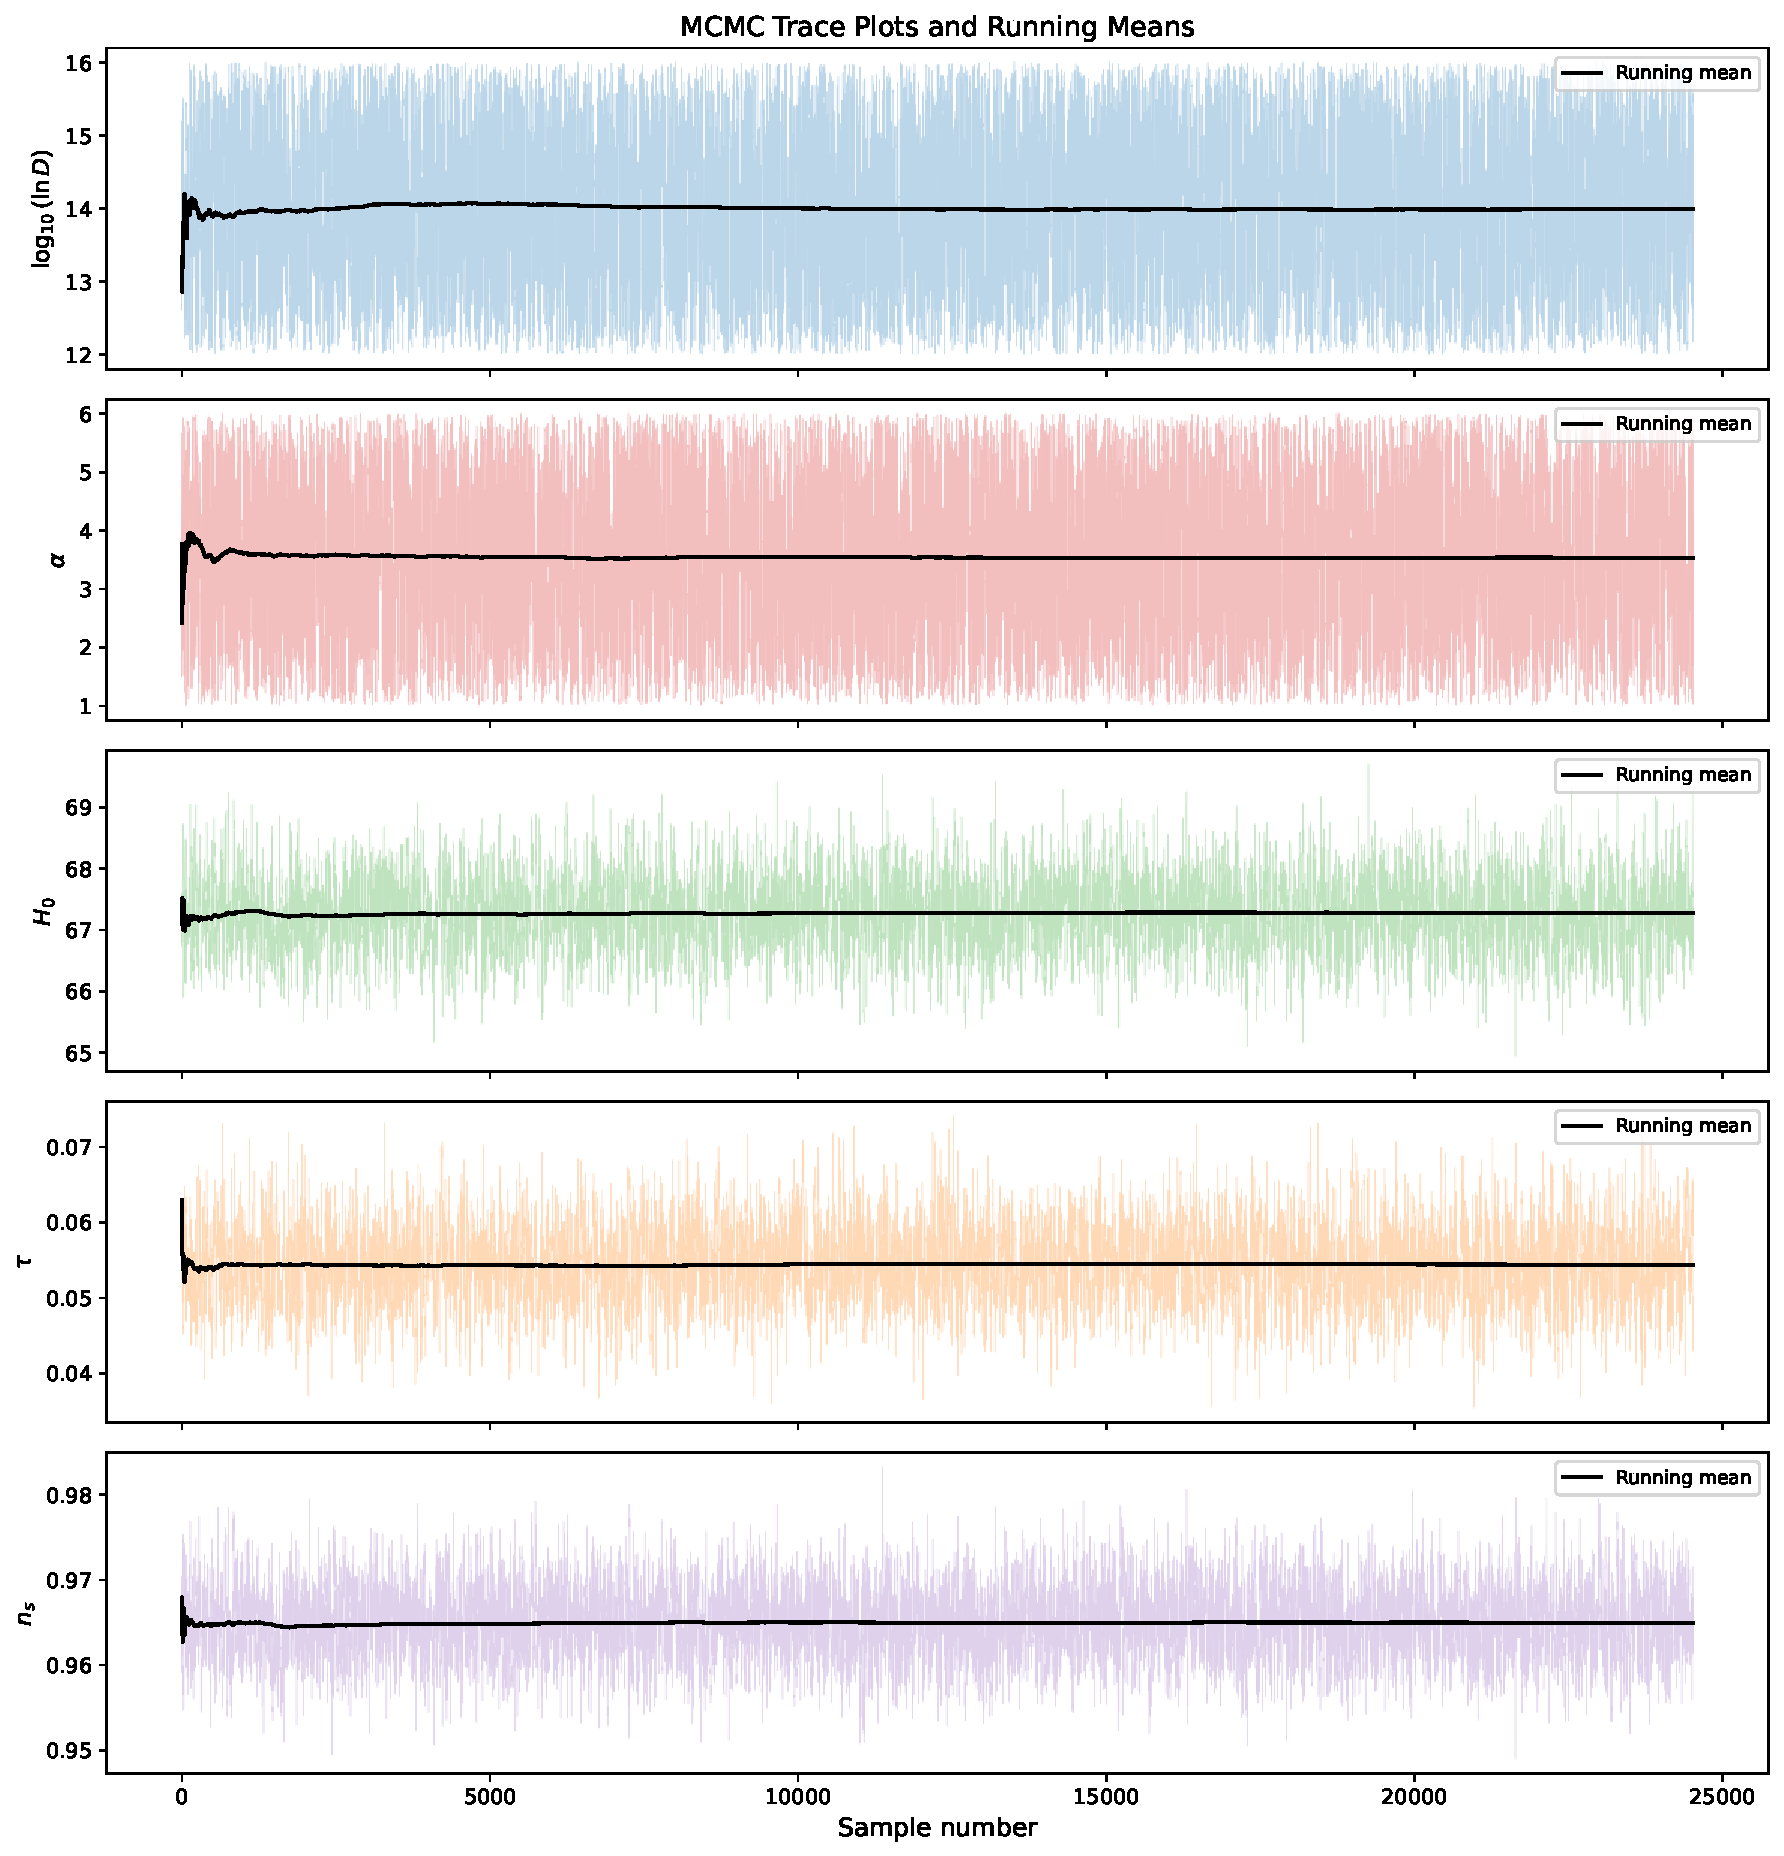
\includegraphics[width=\linewidth]{fig_trace_plots}
  \caption{Trace plots and running weighted means for the five key
    parameters. The CCR parameters explore the full prior range
    uniformly, while the $\Lambda$CDM parameters converge rapidly.}
  \label{fig:trace_plots}
\end{figure}

\begin{figure}[p]
  \centering
  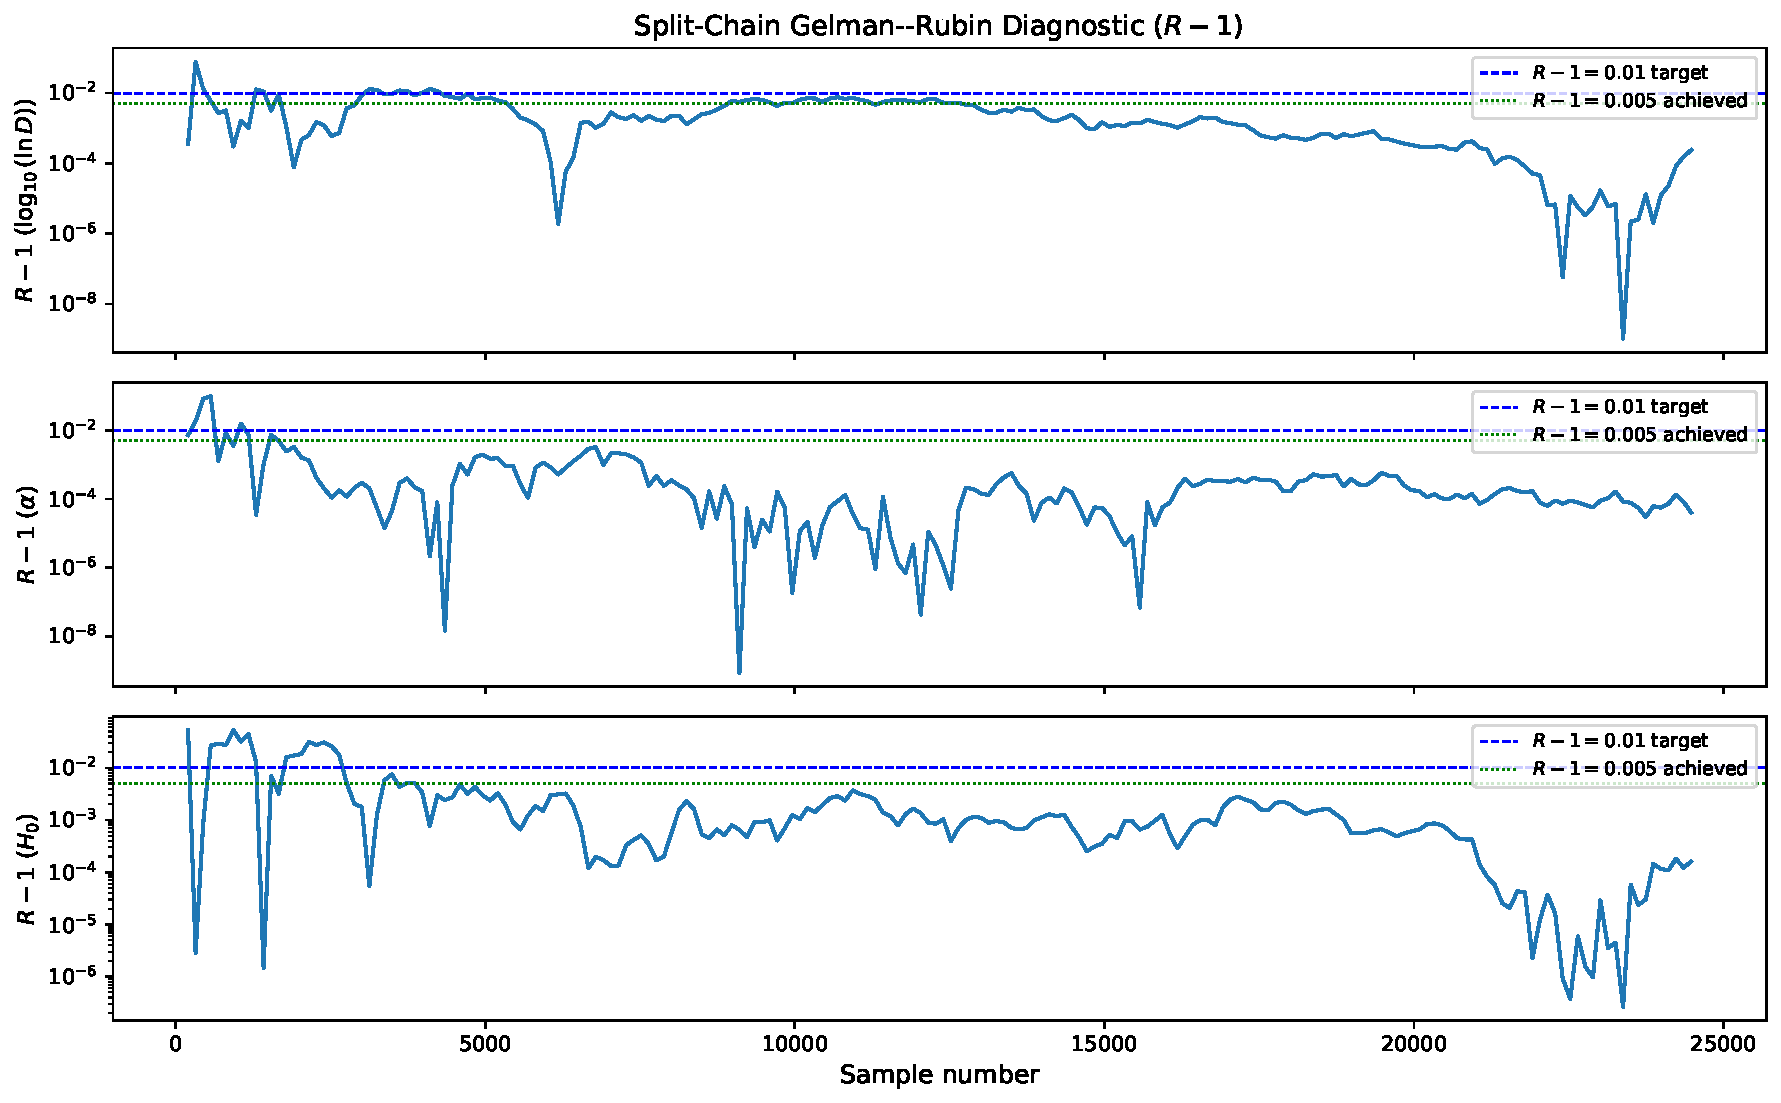
\includegraphics[width=\linewidth]{fig_gelman_rubin}
  \caption{Split-chain Gelman--Rubin diagnostic $R - 1$ as a function
    of sample number. The dashed line marks the $R - 1 = 0.01$ target.
    All parameters fluctuate near or below $R - 1 = 0.01$ for the
    majority of the chain, with a final value of $R - 1 < 0.005$.}
  \label{fig:gelman_rubin}
\end{figure}

\begin{figure}[p]
  \centering
  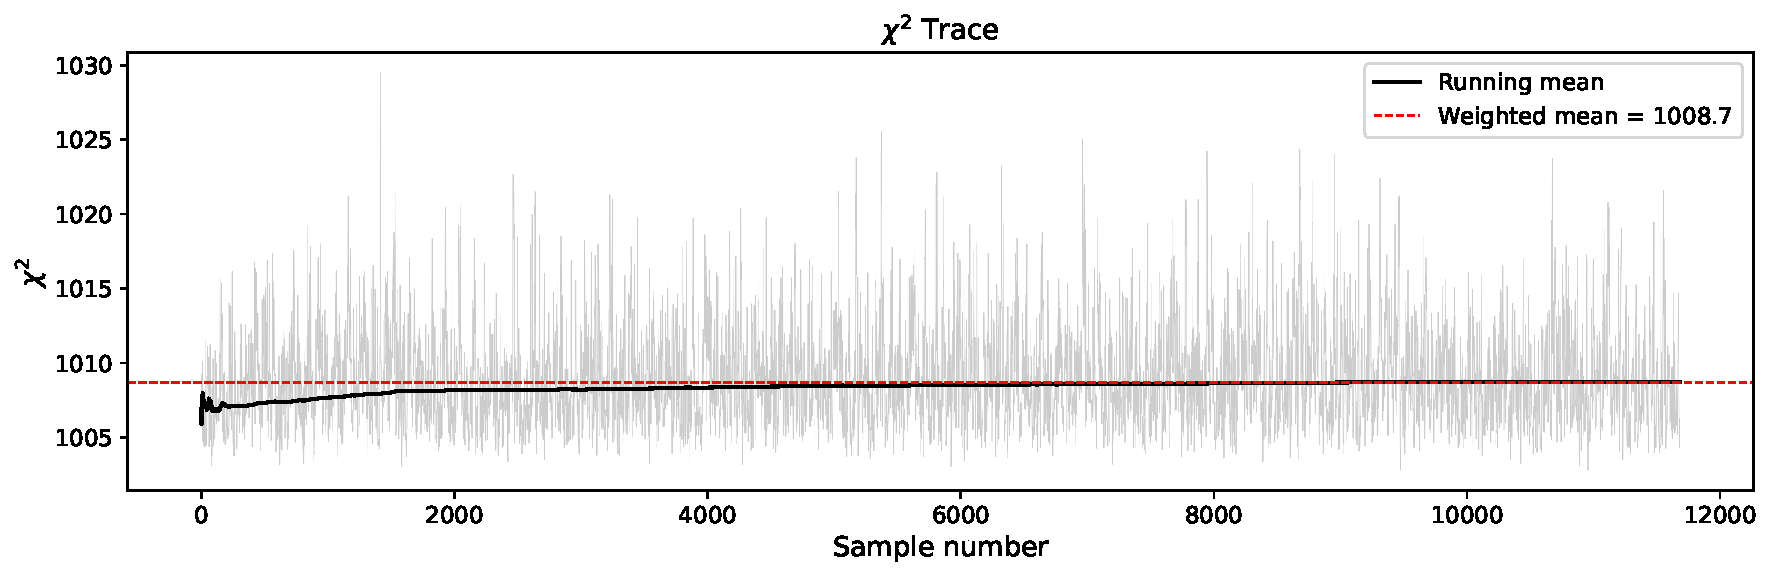
\includegraphics[width=\linewidth]{fig_chi2_trace}
  \caption{$\chi^2$ trace plot. The running mean (black) stabilises at
    $\langle\chi^2\rangle = 1008.9$; the minimum is
    $\chi^2_{\min} = 1002.6$.}
  \label{fig:chi2_trace}
\end{figure}


% ============================================================
% APPENDIX C — Numerical Validation
% ============================================================
\section{Numerical validation}
\label{app:validation}

\paragraph{$\Lambda$CDM recovery.}
Figure~\ref{fig:lcdm_recovery} (upper panel) shows the fractional
difference $|\Delta C_\ell^{TT}/C_\ell^{TT}|$ between the
CCR-modified and standard $\Lambda$CDM spectra for increasing values
of $\ln D$. The results confirm the expected limiting behaviour:

\begin{center}
\begin{tabular}{ccc}
  \hline\hline
  $\ln D$ & $k_c$ [Mpc$^{-1}$] & $\max|\Delta C_\ell^{TT}/C_\ell^{TT}|$ \\
  \hline
  $10^{14}$ & $2.3\times 10^{-4}$ & $2.7\times 10^{-1}$ \\
  $10^{15}$ & $7.3\times 10^{-5}$ & $1.6\times 10^{-2}$ \\
  $10^{16}$ & $2.3\times 10^{-5}$ & $2.2\times 10^{-4}$ \\
  $10^{17}$ & $7.3\times 10^{-6}$ & $1.8\times 10^{-6}$ \\
  $10^{18}$ & $2.3\times 10^{-6}$ & $2.8\times 10^{-11}$ \\
  \hline\hline
\end{tabular}
\end{center}

\noindent
For $\ln D = 10^{16}$ (the upper edge of our prior range), the maximum
fractional deviation is $2.2\times 10^{-4}$, confirming that the
$\Lambda$CDM limit is recovered to high precision. For $\ln D \geq 10^{17}$,
the deviation drops below $10^{-5}$ across all multipoles.

\paragraph{$k$-grid convergence.}
Figure~\ref{fig:lcdm_recovery} (lower panel) compares the TT power
spectrum computed with $n_k = 500$, 1000, and 1500 $k$-grid points
against a reference computation with $n_k = 2000$, for
$\ln D = 2\times 10^{14}$ and $\alpha = 2$. The fractional differences
are below $10^{-5}$ for $n_k \geq 500$, confirming that our fiducial
choice of $n_k = 1500$ is more than adequate.

\begin{figure}[p]
  \centering
  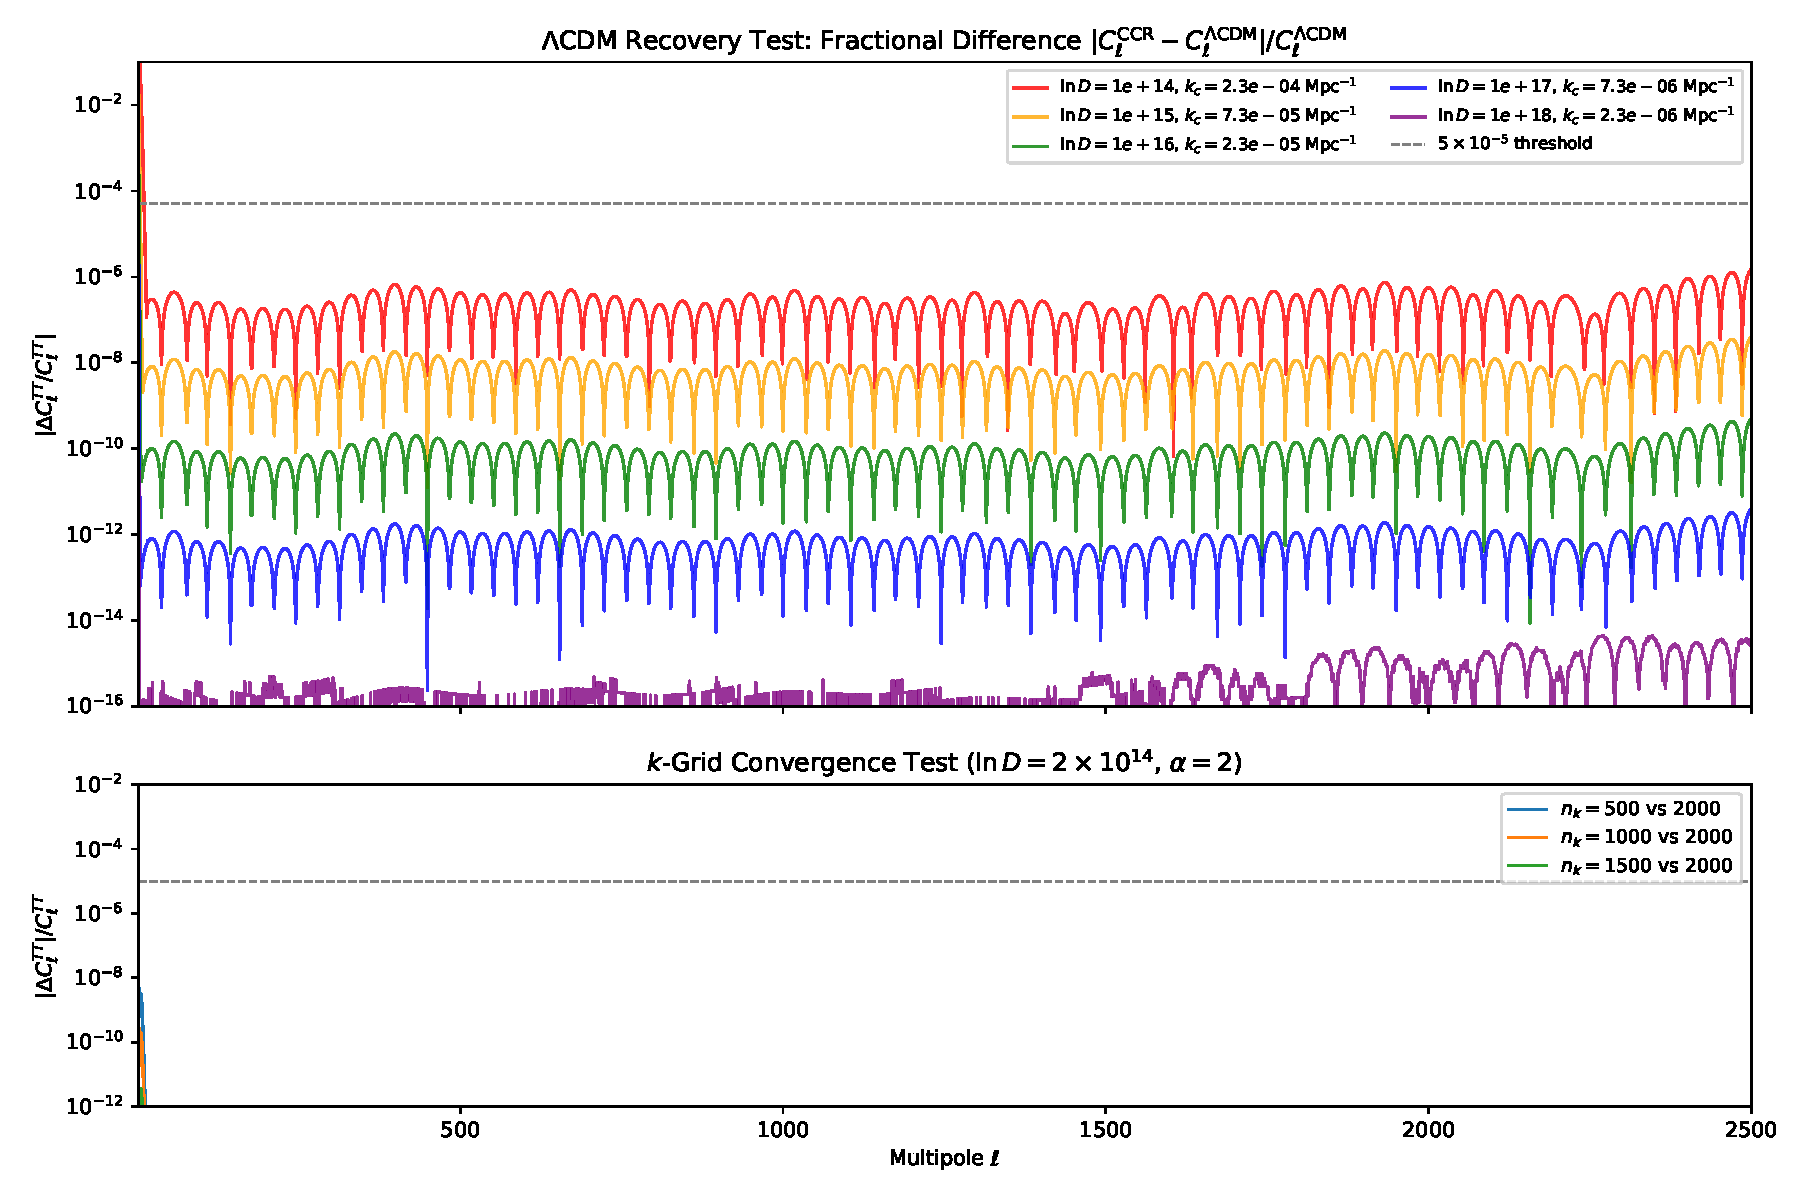
\includegraphics[width=\linewidth]{fig_lcdm_recovery}
  \caption{\textbf{Upper:} $\Lambda$CDM recovery test. Fractional
    difference between CCR and $\Lambda$CDM $C_\ell^{TT}$ for
    increasing $\ln D$. The dashed line marks the
    $5\times 10^{-5}$ threshold.
    \textbf{Lower:} $k$-grid convergence test for
    $\ln D = 2\times 10^{14}$, comparing $n_k = 500$, 1000, 1500
    against a reference with $n_k = 2000$. All grids agree to better
    than $10^{-5}$.}
  \label{fig:lcdm_recovery}
\end{figure}

% ============================================================
% Bibliography
\begin{thebibliography}{99}

\bibitem{Chronis:2026}
N.~Chronis and N.~Sifakis,
\textit{Conditional Cosmological Recurrence in Finite Hilbert Spaces and Holographic Bounds Within Causal Patches},
Universe \textbf{12}(1) (2026) 10,
\href{https://doi.org/10.3390/universe12010010}{doi:10.3390/universe12010010}.

\bibitem{Contaldi:2003}
C.~R.~Contaldi, M.~Peloso, L.~Kofman, and A.~Linde,
\textit{Suppressing the Lower Multipoles in the CMB Anisotropies},
JCAP \textbf{07} (2003) 002
[\href{https://arxiv.org/abs/astro-ph/0309000}{astro-ph/0309000}].

\bibitem{Bunch:1978}
T.~S.~Bunch and P.~C.~W.~Davies,
\textit{Quantum Field Theory in de~Sitter Space: Renormalization by Point Splitting},
Proc.\ R.\ Soc.\ Lond.\ A \textbf{360} (1978) 117.

\bibitem{Bekenstein:1973}
J.~D.~Bekenstein,
\textit{Black Holes and Entropy},
Phys.\ Rev.\ D \textbf{7} (1973) 2333.

\bibitem{Hawking:1975}
S.~W.~Hawking,
\textit{Particle Creation by Black Holes},
Commun.\ Math.\ Phys.\ \textbf{43} (1975) 199.

\bibitem{Gibbons:1977}
G.~W.~Gibbons and S.~W.~Hawking,
\textit{Cosmological Event Horizons, Thermodynamics, and Particle Creation},
Phys.\ Rev.\ D \textbf{15} (1977) 2738.

\bibitem{Mukhanov:2005}
V.~F.~Mukhanov,
\textit{Physical Foundations of Cosmology},
Cambridge University Press (2005).

\bibitem{Birrell:1982}
N.~D.~Birrell and P.~C.~W.~Davies,
\textit{Quantum Fields in Curved Space},
Cambridge University Press (1982).

\bibitem{Baumann:2009}
D.~Baumann,
\textit{TASI Lectures on Inflation},
[\href{https://arxiv.org/abs/0907.5424}{arXiv:0907.5424}].

\bibitem{Ryden:2017}
B.~Ryden,
\textit{Introduction to Cosmology},
2nd ed., Cambridge University Press (2017).

\bibitem{Kolb:1990}
E.~W.~Kolb and M.~S.~Turner,
\textit{The Early Universe},
Addison-Wesley (1990).

\bibitem{Planck:2018inflation}
Planck Collaboration,
\textit{Planck 2018 Results. X. Constraints on Inflation},
A\&A \textbf{641} (2020) A10
[\href{https://arxiv.org/abs/1807.06211}{arXiv:1807.06211}].

\bibitem{Planck:2018params}
Planck Collaboration,
\textit{Planck 2018 Results. VI. Cosmological Parameters},
A\&A \textbf{641} (2020) A6
[\href{https://arxiv.org/abs/1807.06209}{arXiv:1807.06209}].

\bibitem{Lewis:1999}
A.~Lewis, A.~Challinor, and A.~Lasenby,
\textit{Efficient Computation of CMB Anisotropies in Closed FRW Models},
Astrophys.\ J.\ \textbf{538} (2000) 473
[\href{https://arxiv.org/abs/astro-ph/9911177}{astro-ph/9911177}].

\bibitem{Ashtekar:2011}
A.~Ashtekar and D.~Sloan,
\textit{Loop Quantum Cosmology and Slow Roll Inflation},
Phys.\ Lett.\ B \textbf{694} (2011) 108
[\href{https://arxiv.org/abs/0912.4093}{arXiv:0912.4093}].

\bibitem{Agullo:2013}
I.~Agullo, A.~Ashtekar, and W.~Nelson,
\textit{A Quantum Gravity Extension of the Inflationary Scenario},
Phys.\ Rev.\ Lett.\ \textbf{109} (2012) 251301
[\href{https://arxiv.org/abs/1209.1609}{arXiv:1209.1609}].

\bibitem{Efstathiou:2004}
G.~Efstathiou,
\textit{A Maximum Likelihood Analysis of the Low CMB Multipoles from WMAP},
Mon.\ Not.\ R.\ Astron.\ Soc.\ \textbf{346} (2003) L26
[\href{https://arxiv.org/abs/astro-ph/0306431}{astro-ph/0306431}].

\bibitem{Torrado:2021}
J.~Torrado and A.~Lewis,
\textit{Cobaya: Code for Bayesian Analysis of an Expanding Universe},
JCAP \textbf{05} (2021) 057
[\href{https://arxiv.org/abs/2005.05290}{arXiv:2005.05290}].

\bibitem{Planck:2018likelihood}
Planck Collaboration,
\textit{Planck 2018 Results. V. Power Spectra and Likelihoods},
A\&A \textbf{641} (2020) A5
[\href{https://arxiv.org/abs/1907.12875}{arXiv:1907.12875}].

\bibitem{Dickey:1971}
J.~M.~Dickey,
\textit{The Weighted Likelihood Ratio, Linear Hypotheses on Normal Location Parameters},
Ann.\ Math.\ Statist.\ \textbf{42} (1971) 204.

\bibitem{Kass:1995}
R.~E.~Kass and A.~E.~Raftery,
\textit{Bayes Factors},
J.\ Amer.\ Statist.\ Assoc.\ \textbf{90} (1995) 773.

\bibitem{Liddle:2007}
A.~R.~Liddle,
\textit{Information Criteria for Astrophysical Model Selection},
Mon.\ Not.\ R.\ Astron.\ Soc.\ \textbf{377} (2007) L74
[\href{https://arxiv.org/abs/astro-ph/0701113}{astro-ph/0701113}].

\bibitem{Starobinsky:1992}
A.~A.~Starobinsky,
\textit{Spectrum of Adiabatic Perturbations in the Universe when There Are Singularities in the Inflation Potential},
JETP Lett.\ \textbf{55} (1992) 489.

\bibitem{Ratra:1995}
B.~Ratra and P.~J.~E.~Peebles,
\textit{Inflation in an Open Universe},
Phys.\ Rev.\ D \textbf{52} (1995) 1837.

\bibitem{LiteBIRD:2022}
LiteBIRD Collaboration,
\textit{Probing Cosmic Inflation with the LiteBIRD Cosmic Microwave Background Polarization Survey},
PTEP \textbf{2023} (2023) 042F01
[\href{https://arxiv.org/abs/2202.02773}{arXiv:2202.02773}].

\bibitem{CMBS4:2016}
CMB-S4 Collaboration,
\textit{CMB-S4 Science Book, First Edition},
[\href{https://arxiv.org/abs/1610.02743}{arXiv:1610.02743}] (2016).

\bibitem{Banks:2000}
T.~Banks,
\textit{Cosmological Breaking of Supersymmetry, or Little Lambda Goes Back to the Future II},
[\href{https://arxiv.org/abs/hep-th/0007146}{hep-th/0007146}] (2000).

\bibitem{Banks:2001}
T.~Banks and W.~Fischler,
\textit{M-Theory Observables for Cosmological Space-Times},
[\href{https://arxiv.org/abs/hep-th/0102077}{hep-th/0102077}] (2001).

\bibitem{Bousso:2000}
R.~Bousso,
\textit{The Holographic Principle},
Rev.\ Mod.\ Phys.\ \textbf{74} (2002) 825
[\href{https://arxiv.org/abs/hep-th/0203101}{hep-th/0203101}].

\bibitem{Schwarz:2016}
D.~J.~Schwarz, C.~J.~Copi, D.~Huterer, and G.~D.~Starkman,
\textit{CMB Anomalies after Planck},
Class.\ Quant.\ Grav.\ \textbf{33} (2016) 184001
[\href{https://arxiv.org/abs/1510.07929}{arXiv:1510.07929}].

\bibitem{Trotta:2008}
R.~Trotta,
\textit{Bayes in the Sky: Bayesian Inference and Model Selection in Cosmology},
Contemp.\ Phys.\ \textbf{49} (2008) 71
[\href{https://arxiv.org/abs/0803.4089}{arXiv:0803.4089}].

\bibitem{Susskind:2003}
L.~Susskind,
\textit{The Anthropic Landscape of String Theory},
[\href{https://arxiv.org/abs/hep-th/0302219}{hep-th/0302219}] (2003).

\bibitem{Dyson:2002}
L.~Dyson, M.~Kleban, and L.~Susskind,
\textit{Disturbing Implications of a Cosmological Constant},
JHEP \textbf{10} (2002) 011
[\href{https://arxiv.org/abs/hep-th/0208013}{hep-th/0208013}].

\bibitem{Hogan:2002}
C.~J.~Hogan,
\textit{Holographic Discreteness of Inflationary Perturbations},
Phys.\ Rev.\ D \textbf{66} (2002) 023521
[\href{https://arxiv.org/abs/astro-ph/0201020}{astro-ph/0201020}].

\bibitem{Hogan:2005}
C.~J.~Hogan,
\textit{Observational Tests of Planck-Scale Discreteness},
AIP Conf.\ Proc.\ \textbf{743} (2005) 138.

\bibitem{Enqvist:2002}
K.~Enqvist and M.~S.~Sloth,
\textit{Possible Signatures of the Trans-Planckian Physics in the CMB},
Nucl.\ Phys.\ B \textbf{626} (2002) 395
[\href{https://arxiv.org/abs/hep-ph/0109210}{hep-ph/0109210}].

\bibitem{DESI:2024}
DESI Collaboration,
\textit{DESI 2024 VI: Cosmological Constraints from the
Measurements of Baryon Acoustic Oscillations},
JCAP \textbf{02} (2025) 021
[\href{https://arxiv.org/abs/2404.03002}{arXiv:2404.03002}].

\bibitem{DESI:2025}
DESI Collaboration,
\textit{DESI DR2: Measurements of Baryon Acoustic Oscillations
and Cosmological Constraints},
Phys.\ Rev.\ D \textbf{112} (2025) 083515 [arXiv:2503.14738].

\bibitem{Campeti:2025}
P.~Campeti, E.~Komatsu, C.~Baccigalupi, and
M.~Ballardini,
\textit{Inflation at the End of 2025: Constraints on $r$
and $n_s$ Using the Latest CMB and BAO Data},
arXiv:2512.10613 (2025).

\bibitem{Chandrasekaran:2023}
V.~Chandrasekaran, R.~Longo, G.~Penington, and E.~Witten,
\textit{An Algebra of Observables for de Sitter Space},
JHEP \textbf{02} (2023) 082 [arXiv:2206.10780].

\bibitem{Chakraborty:2024}
T.~Chakraborty, J.~Chakravarty, V.~Godet, P.~Kraus,
and A.~Sivakumar,
\textit{The Hilbert Space of de Sitter Quantum Gravity},
JHEP \textbf{01} (2024) 132 [arXiv:2303.16315].

\bibitem{Tajima:2024}
H.~Tajima and Y.~Nambu,
\textit{Stochastic inflation and entropy bound in de Sitter spacetime},
[\href{https://arxiv.org/abs/2405.10837}{arXiv:2405.10837}] (2024).

\bibitem{Ghigna:2024}
T.~Ghigna et al. (LiteBIRD Collaboration),
\textit{The LiteBIRD mission to explore cosmic inflation},
SPIE Astronomical Telescopes + Instrumentation 2024
[\href{https://arxiv.org/abs/2406.02724}{arXiv:2406.02724}] (2024).

\end{thebibliography}

\end{document}